% !TEX encoding = UTF-8 Unicode
\documentclass{textile}

\usepackage{amsmath}

\usepackage[sorting=nyt,style=numeric-comp]{biblatex}
\bibliography{whitepaper}

%\copyrightyear{2009} \vol{00} \issue{0} \DOI{000}

% for full width figures\
\usepackage{lipsum}% http://ctan.org/pkg/lipsum
\usepackage{graphicx}% http://ctan.org/pkg/graphicx

% random
\usepackage[utf8]{inputenc} % allow utf-8 input
\usepackage[T1]{fontenc}    % use 8-bit T1 fonts
\usepackage{hyperref}       % hyperlinks
\usepackage{url}            % simple URL typesetting
\usepackage{nicefrac}       % compact symbols for 1/2, etc.

\usepackage{dblfloatfix}    % To enable figures at the bottom of page

% keep footnotes from wrapping pages,
\interfootnotelinepenalty=10000

% trying to keep figures in the right sections instead of pushed to the end
\usepackage[section]{placeins}

% to make paragraph look a bit more like a subsubsubsection
\makeatletter
\renewcommand\paragraph{\@startsection{paragraph}{4}{\z@}%
            {-2.5ex\@plus -1ex \@minus -.25ex}%
            {1.25ex \@plus .25ex}%
            {\normalfont\normalsize\itshape}}
\makeatother
\setcounter{secnumdepth}{3} % how many sectioning levels to assign numbers to
\setcounter{tocdepth}{3}    % how many sectioning levels to show in ToC

% To create tables + create check-marks
\usepackage{booktabs}
\usepackage{colortbl}
\usepackage{multirow}% http://ctan.org/pkg/multirow

\usepackage{array}
\usepackage{tikz}
\def\checkmark{\tikz\fill[scale=0.4](0,.35) -- (.25,0) -- (1,.7) -- (.25,.15) -- cycle;} 

\newcommand\Tstrut{\rule{0pt}{2.6ex}}       % "top" strut
\newcommand\Bstrut{\rule[-0.9ex]{0pt}{0pt}} % "bottom" strut
\newcommand{\TBstrut}{\Tstrut\Bstrut} % top&bottom struts

% column centering special type
\newcolumntype{P}[1]{>{\centering\arraybackslash}p{#1}}
% End table requirements

% Thread ID components fig requirements
\usepackage{stackengine}
% Thread ID equation setup 
\def\textscrm#1{\textrm{\scriptsize#1}}
\stackMath
\def\rldp{1.3ex}
\def\rlht{.8ex}
\def\rlwd{.8pt}
\setstackgap{L}{\rldp}
\def\uvbarR#1{%
  \def\stackalignment{r}\def\stacktype{S}\stackunder[-\rlwd]{%
    \def\stackalignment{c}\def\stacktype{L}\stackunder{#1}{\rule{\rlwd}{\rlht}}%
  }{\setbox0\hbox{$#1$}\rule{.5\wd0}{\rlwd}}%
}
\def\uvbarL#1{%
  \def\stackalignment{l}\def\stacktype{S}\stackunder[-\rlwd]{%
    \def\stackalignment{c}\def\stacktype{L}\stackunder{#1}{\rule{\rlwd}{\rlht}}%
  }{\setbox0\hbox{$#1$}\rule{.5\wd0}{\rlwd}}%
}
\def\uvbar#1#2{%
  \def\stacktype{S}\def\stackalignment{c}\def\useanchorwidth{T}\stackunder[0pt]{%
    \def\stacktype{L}\setbox0\hbox{${}#1{}$}%
    \stackunder[\rldp]{{}#1{}}{\rule{\wd0}{\rlwd}}%
  }{\def\stacktype{S}\stackunder[1pt]{\rule{\rlwd}{\rlht}}{\scriptstyle#2}}%
}
\newcommand\ubar[2]{\uvbarR{\textrm{}}\uvbar{\textrm{#1}}{\textscrm{#2}}%
  \uvbarL{\textrm{}}}
\newcommand\phubar[2]{\uvbarR{\textrm{}}\uvbar{\phantom{\textrm{#1}}}{\textscrm{#2}}%
  \uvbarL{\textrm{}}}

% End thread Id requirements

% double column box
\usepackage{cuted,tcolorbox,lipsum}

% code embeds
\usepackage{listings}
\usepackage{color}

\definecolor{dkgreen}{rgb}{0,0.6,0}
\definecolor{gray}{rgb}{0.5,0.5,0.5}
\definecolor{mauve}{rgb}{0.58,0,0.82}

\lstset{frame=tb,
  language=Go,
  aboveskip=3mm,
  belowskip=3mm,
  showstringspaces=false,
  columns=flexible,
  basicstyle={\small\ttfamily},
  numbers=none,
  numberstyle=\tiny\color{gray},
  keywordstyle=\color{blue},
  commentstyle=\color{dkgreen},
  stringstyle=\color{mauve},
  breaklines=true,
  breakatwhitespace=true,
  tabsize=3
}

% color the json
\lstdefinelanguage{json}{
  basicstyle={\small\ttfamily},
  numbers=none,
    numberstyle=\scriptsize,
    stepnumber=1,
    numbersep=8pt,
    showstringspaces=false,
    breaklines=true,
    frame=lines,
    backgroundcolor=\color{white},
    literate=
     *{0}{{{\color{black}0}}}{1}
      {1}{{{\color{black}1}}}{1}
      {2}{{{\color{black}2}}}{1}
      {3}{{{\color{black}3}}}{1}
      {4}{{{\color{black}4}}}{1}
      {5}{{{\color{black}5}}}{1}
      {6}{{{\color{black}6}}}{1}
      {7}{{{\color{black}7}}}{1}
      {8}{{{\color{black}8}}}{1}
      {9}{{{\color{black}9}}}{1}
      {:}{{{\color{gray}{:}}}}{1}
      {\{}{{{\color{gray}{\{}}}}{1}
      {\}}{{{\color{gray}{\}}}}}{1}
      {[}{{{\color{gray}{[}}}}{1}
      {"}{{{\color{gray}{"}}}}{1}
      {,}{{{\color{gray}{,}}}}{1}
      {]}{{{\color{gray}{]}}}}{1},
}

% bolds "Example X" to match Figure X
\usepackage[labelfont=bf]{caption}
\DeclareCaptionType{example}

\usepackage{trivfloat}
\trivfloat{example}

\usepackage{pagecolor}

\begin{document}
\pagecolor{white}

\title[A protocol and event-sourced database for decentralized user-siloed data]{A protocol and event-sourced database for decentralized user-siloed data}
\author{Pick}
\author{Farmer}
\author{Sutula}
\affiliation{www.textile.io} \email{research@textile.io}
\author{?Gozalishivili others?}
\affiliation{other?} \email{research@textile.io}
\author{Hill}
\affiliation{www.textile.io} \email{contact@textile.io}

\shortauthors{www.textile.io}

\revised{18 September 2019}


%\category{C.2}{Computer Communication Networks}{Computer Networks}
%\category{C.4}{Performance of Systems}{Analytical Models}
%\category{G.3}{Stochastic Processes}{Queueing Systems}
%\terms{Internet Technologies, E-Commerce}
\keywords{Databases; Event Sourcing; IPFS; IPLD}


\begin{abstract}
As the Internet expands, the division between a person's digital and physical existence continues to blur. An emerging issue of concern is that the digital part of a person's life is mainly being captured by apps and stored away from the person's control by the companies building those apps. An alternative, called user-siloed data is one area of research that if implemented successfully, could reverse the flow of value derived from personal data, from apps to users. In this paper, we investigate the data formats, access control, and transfer protocols necessary to build a system for user ownership of large-scale digital datasets. The aim of the proposed system is to help power a new generation of web technologies. Our solution combines a novel use of event sourcing with Interplanetary Linked Data (IPLD) to provide a distributed, scalable, and flexible database solution for decentralized applications.
\end{abstract}

\maketitle

\section{Introduction}

Compared to their predecessors, modern cloud-based apps and services provide an extremely high level of convenience. Users can entirely forget about the risk of data loss and enjoy seamless access to their apps across multiple devices. This convenience is now expected, but has come at the cost of additional consequences for users. One such consequence is that many of the same development patterns that bring convenience (e.g., single sign-on, minimal encryption, centralized servers, and databases) also enable or even require data hoarding by the apps. While collecting large amounts of users' data can create value for the companies building apps (e.g., app telemetry, predictive tools, or even new revenue streams), that value flows mostly in one direction; Apps collect, process and benefit from a user's private data, but users rarely have access to the original data or the new insights that come from it. Additionally,  the data may not be readily accessible to other apps and services. This is app-siloed data.

While companies collecting user data may not be itself a significant problem, it has been shown that over time company incentives often shift from providing value to users to extracting value from users \cite{dixonWhyDecentralizationMatters2018}. When this incentive shift happens for companies that have also been hoarding user data, that data may be a new source of value or even revenue for the company. It may be possible to stop this trend through extreme privacy measures, government intervention/legislation, or by boycotting companies that collect any form of data. Ideally, there is an alternative approach that allows individuals to capture the value of their data and still allow developers to build new interfaces and experience on top of this data. This approach is called user-siloed data and it fundamentally separates apps from their user's data.

One of the most exciting aspects of user-siloed data is the the ability to build data-driven apps and services while users remain in control of their own data. Other projects have identified app silo-ed data as a problem \cite{bernersLee_readwrite_2013,de_montjoye_trusted_2012}, and some have identified user-siloed data as a solution \cite{sambraSolidPlatformDecentralized2016}. However, none so far have provided a sufficiently interoperable protocol for scalable storage and transmission of user-siloed application data. This is the key to building great applications on user-siloed data.

In this paper, we study existing technologies that could be used to build a network for user-siloed data. We outline six challenge areas: flexible data format, efficient synchronization, conflict resolution, access-control, scalable storage, and network communication. Based on our findings, we propose a novel architecture for event sourcing with Interplanetary Linked Data (IPLD), designed to store, share, and host user-sioled datasets at scale. Our proposed design leverages new and existing protocols to solve major challenges involved with building a secure and distributed network for user data while at the same time providing the flexibility and scalability required by today's applications. 


\section{Background}
\label{sec:Background}

We now describe some of the technologies and concepts motivating the design of our novel decentralized database system. We highlight some of the advantages and lessons that can be learned from event-sourcing and discuss drawbacks to using these approaches in decentralized systems. We provide an overview of some important technologies related to IPFS that make it possible to rethink event sourcing in a decentralized network. Finally, we cover challenges of security and access control on an open and decentralized network and discuss how they are used in popular databases external to IPFS. 

\subsection{Data Synchronization}

\subsubsection{CQRS, Event Sourcing, and Logs}\label{sec:cqrs}

When developing large-scale software systems, it is common to store data in a relational database management system (RDBMS). To model realistic systems, this type of framework often requires complex techniques for mapping data between domain models and database tables, where the same data model is used to both query and update a database. A powerful alternative is to use a set of append only logs to model the state of an object simply by applying its change sequence in the correct order. This concept can be expressed succinctly by the state machine approach \cite{schneiderImplementingFaulttolerantServices1990}: if two identical, deterministic processes begin in the same state and get the same inputs in the same order, they will produce the same output and end in the same state. This is a powerful concept baked into a simple structure, and is at the heart of many distributed database systems \cite{jaykrepsLogWhatEvery2013}.

\begin{definition} (Logs or Append-only log). A log is a registry of database transactions that is read sequentially (normally ordered by time) from beginning to end. In distributed systems, logs are often treated as append-only, where changes or updates can only be added to the set and never removed.  \end{definition} \label{def:Logs}

In modern applications it is critical to have reliable mechanisms for publishing updates and events (i.e., to support event-driven architectures), scalability (optimized write and read operations), forward-compatible application updates (e.g., code changes, retroactive events, and others), auditing systems, etc. To support such requirements, developers have begun to utilize event sourcing and command query responsibility segregation (CQRS) patterns \cite{bettsExploringCQRSEvent2013}, relying on append only logs to support immutable state histories. Indeed, a number of commercial and open source software projects have emerged in recent years that facilitate event sourcing and CQRS-based applications, including Event Store \cite{EventStore}, Apache Kafaka \cite{ApacheKafka} and Samza \cite{ApacheSamza}, among others (see \cite{kleppmannDesigningDataintensiveApplications2017}). 

\begin{definition} (Command query responsibility segregation). Command query responsibility segregation or CQRS is a design pattern whereby reads and writes are separated into different models, using commands to write data, and queries to read data \cite{martinfowlerCQRS2011}. \end{definition}

\begin{definition} (Event sourcing). Event sourcing (ES) is a design pattern for persisting the state of an application as an append-only log of state-changing events. \end{definition}

ES is particularly useful in contexts where system components are distributed or decentralized, such as in decentralized applications (DApps). This is because the design of systems that use event sourcing often necessitate infrastructure for brokering messages between loosely coupled software components and services. This feature will become increasingly important as we outline background concepts related to data synchronization in the following sections. 

A key principal of ES and append only logs is that all changes to application state are stored as a sequence of events. Because any given state is simply the result of a series of atomic updates, the log can be used to reconstruct past states or process retroactive updates \cite{fowlerEventSourcing}. The same principal means a log can be viewed as a mechanism to support an infinite number of valid state interpretations (Section  \ref{sec:ViewsProjections}). In other words, with minimal conformity, a single log can model multiple application states \cite{microsoftcorporationAzureApplicationArchitecture}.

\subsubsection{Views \& Projections} \label{sec:ViewsProjections}

\begin{definition}  (View). A (typically highly de-normalized) read-only model of the data. Views are tailored to the interfaces and display requirements of the application, which helps to maximize both display and query performance. Views that are backed by a database or filesystem-optimized access are referred to as materialized views. \end{definition}

\begin{definition} (Projection). An event handler and corresponding reducer/fold function used to build and maintain a view from a set of (filtered) events. While projections may lead to the generation of new events, their reducer should be a pure function (see \cite{eventsourceEventSourcingBasics} and \cite{reduxGettingStartedRedux} for examples from existing systems). \end{definition}

In CQRS and ES, the separation of write operations from read operations is a powerful concept. It allows developers to define views into the underlying data that are best suited for the use case or user interface they are building. Multiple views can be built from the same underlying event log, and they can be quite different from one another.

Views themselves are enabled by projections\footnote{Terminology in this section may differ from some other examples of ES and CQRS patterns, but reflects the underlying architecture and designs that the Textile team will elaborate on in \ref{sec:ThreadsProtocol}}. Projections can be thought of as transformations or reducers that are applied to each event in a stream of events. They update the data backing the views, be this in memory, or persisted to a database. In a distributed setting, it may be necessary for projections to define and operate as eventually consistent data structures, to ensure all peers operating on the same stream of events have a consistent representation of the data.

\subsubsection{Eventual Consistency} \label{sec:EventualConsistency}

The CAP theorem \cite{brewerRobustDistributedSystems2000,gilbertBrewerConjectureFeasibility2002a} states that a distributed database can guarantee only two of the following three promises at the same time: consistency (i.e., that every read receives the most recent write or an error), availability (i.e., that every request receives a (possibly out-of-date) non-error response, and partition tolerance (i.e., that the system continues to operate despite an arbitrary number of messages being dropped (or delayed) by the network). As such, many distributed systems are now designed to provide availability and partition tolerance by trading consistency for eventual consistency. Eventual consistency allows state replicas to diverge temporarily, but eventually arrive back to the same state again. While an active area of research, designing systems with provable eventual consistency guarantees remains challenging \cite{shapiroComprehensiveStudyConvergent2011a,almeidaDeltaStateReplicated2018}.


\begin{definition} (CRDT). A conflict-free replicated data type (CRDT) assures eventual consistency through optimistic replication (i.e. all new updates are allowed) and eventual merging. CRDTs rely on data structures that are mathematically guaranteed to resolve concurrent updates the same way regardless of the order those events were received. \end{definition} \label{def:CRDT}

How a system provides eventual consistency is often decided based on the intended use of the system. Two well-documented categories of solutions include logs (Definition  \ref{def:Logs}), sequences of deterministic changes, and CRDTs (Definition  \ref{def:CRDT}). Logs work best when there is only a single-writer or complete event causality is known. In many distributed systems with multiple log writers, a minimum requirement for synchronization through logs is that the essential order of events is respected and can be determined \cite{schwarzDetectingCausalRelationships1994,katzInterleavingSetTemporal1990}. For these cases, logical clocks are a useful tool for eventual consistency and total ordering \cite{kulkarniLogicalPhysicalClocks2014}. However, some scenarios (e.g., temporarily missing events, or ambiguous order) can force a replica into a state that cannot be later resolved without costly recalculation. In specific cases, CRDTs can provide an alternative to log-based consensus (see below). 

\subsubsection{Logical Clocks}\label{sec:LogicalClocks}

In a distributed system, where multiple machines, each with an independent clock, are creating events, local timestamps can't be used to construct global event causality. Machine clocks are never perfectly synchronized \cite{lamportTimeClocksOrdering1978}, meaning that one machine's concept of "now" is not necessarily the same as another machine's. Machine speed, network speed, and other factors compound the issue. For this reason, simple wall-clock time does not provide a sufficient notion of order in a distributed system. Alternatives to wall-clock time exist to help distributed systems achieve eventual consistency. Examples include various logical clocks (Lamport \cite{lamportTimeClocksOrdering1978} Schwartz \cite{schwarzDetectingCausalRelationships1994}, and Bloom \cite{ramabajaBloomClock2019}, Hybrid variants \cite{kulkarniLogicalPhysicalClocks2014}, etc), which use counter-based time-stamping to provide partial ordering. 

Cryptographically linked events can also represent a clock (See Section \ref{sec:merkleclocks}). One such example is called the Merkle-Clock \cite{sanjuanMerkleCRDTs2019}. The Merkle-Clock relies on properties of a Merkle-DAG to provide strict partial ordering between events, which has limitations \cite[sec. 4.3]{sanjuanMerkleCRDTs2019}:

\begin{quote}
Merkle-Clocks represent a strict partial order of events. Not all events in the system can be compared and ordered. For example, when having multiple heads, the Merkle-Clock cannot say which of the events happened before.
\end{quote}

\subsubsection{Conflict-Free Replicated Data Types}\label{sec:CRDTs}

In distributed models that use clock-based ordering as described above, a replica can arrive in a state that will require conflict resolution through consensus or rollback. Those operations can be expensive, having adverse effects on the scalability of distributed systems, especially ones attempting to synchronize an application state. 

CRDTs (Definition \ref{def:CRDT}) are one way to achieve strong eventual consistency, where once all replicas have received the same events, they will arrive at the same final state, \emph{regardless of ordering}\footnote{Though non-commutative CRDTs may require a specific ordering of events in certain cases \cite{sanjuanMerkleCRDTs2019}}. A review of the types of possible CRDTs is beyond the scope of this paper, however, it is important to note their role in eventually consistent systems and how they relate to clock-based event ordering. See for example \cite{enesSingleWriterPrincipleCRDT2017,sanjuanMerkleCRDTs2019} for informative reviews of these types of data structures.

Whether a system (e.g., an app) uses a CRDT or a clock-based sequence of events is entirely dependent on the use-case and final data model. While CRDTs may seem superior (and are currently a popular choice among decentralized systems), it is not possible to model every system as a CRDT. Additionally, the simplicity of clock-based sequencing often makes it easier to leverage in distributed systems where data conflicts will only rarely arise. Lastly, logs and CRDTs are not mutually exclusive and can be used together or as different stages of a larger system.

\subsection{Content-based addressing}

Internet application architecture today is often designed as a system of clients (users) communicating to endpoints (hosts). Communication between clients and endpoints (servers) happens via the TCP/IP protocol stack and therefore largely relies on a mechanism referred to as location-based addressing. Location-based addressing, where the client makes a request that is routed to a specific endpoint based on prior knowledge (e.g., the domain name or IP address), works relatively well for many use-cases. However, there are many reasons why addressing content by location is problematic, such as duplication of storage, inefficient use of bandwidth, link rot, centralized control, and authentication issues. An alternative to location addressing, called content addressing may provide a solution to those problems. Content addressing is where the content itself is used to create an address and retrieve that content from a network \cite{mortContentBasedAddressing2012}.

\subsubsection{IPFS \& Content-based addressing}

There are a number of systems that utilize content addressing to access content and information (e.g. Git, IPFS, Perkeep, Tahoe-LAFS), and there is an active body of literature covering its design and implementation \cite{benetIPFSContentAddressed2014,selimi_tahoeLafs_2014,rhea_fast_2008}. The Interplanetary File System (IPFS) --- which is a set of protocols to create a content-addressed, peer-to-peer filesystem \cite{benetIPFSContentAddressed2014} --- is one such system. In IPFS, the address for any content is determined based on a cryptographic hash of the content itself. In practice, the IPFS Content IDentifier (CID) is a multihash, which is a self-describing ``protocol for differentiating outputs from various well-established cryptographic hash functions, addressing size + encoding considerations\footnote{\url{https://multiformats.io/}}''. That addressing system confers several benefits to the network, including tamper resistance (we can be confident that a given piece of content has not been modified en route if its hash matches what we were expected/requested) and de-duplication (because the same content from different peers will produce the same hash address). Additionally, IPFS content addresses are immutable and universally unique.

\begin{figure}
  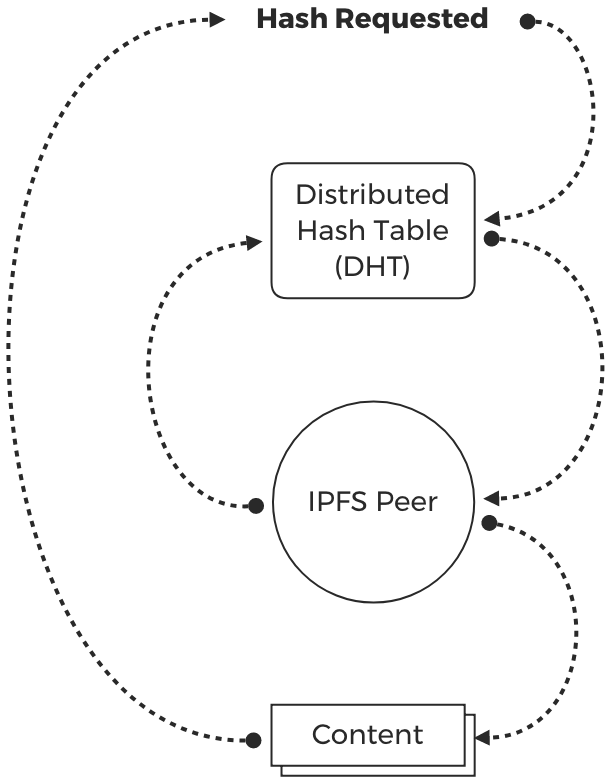
\includegraphics[width=\linewidth]{figures/Hash_Request.png}
  \caption{The cryptographic hash of content is used to make a request to the network of IPFS peers. Using the built-in routing mechanisms and the distributed hash table, a peer(s) hosting the requested content is identified and content is returned. }
  \label{fig:contentaddressing}
\end{figure}

While content addressing doesn't tell you how to get a file, IPFS (via libp2p\footnote{\url{https://libp2p.io/}}) provides a system for moving files across the network.  On the IPFS network, a client who wants specific content requests the CID from the network of IPFS hosts. The client's request is routed to the first host capable of fulfilling the request (i.e., the first host that is actively storing the content behind the given CID). The IPFS network can be seen as a distributed file system, with all of the benefits that come with this type of file system design.

\subsubsection{IPLD}

As discussed above, IPFS uses the cryptographic hash of a given piece of content to define its content address (see \cite{benetIPFSContentAddressed2014} for details on this process). However, in order to provide standards for accessing content-addressable data (on the web or elsewhere), it is necessary to define a common format or specification. In IPFS (and others \cite[e.g.,]{protocollabsFilecoinDecentralizedStorage2017} MORE NEEDED), this common data format is called Interplanetary Linked Data (IPLD)\footnote{\url{https://ipld.io/}}. As the name suggests, IPLD is based on principals of linked data \cite{berners-leeLinkedData2009,bizerLinkedDataStory2011} with the added capabilities of a content-addressing storage network. 

IPLD is used to publish linked data (subject, predicate, object triples in the linked data world \cite{heathLinkedDataEvolving2011}) spread across different hosts, and where everything (e.g., entities, predicates, data sources) uses content addresses as unique identifiers. To form its structure, IPLD implements a Merkle DAG, or directed acyclic graph\footnote{Other examples of Dags include the Bitcoin Blockchain or a Git version history.}. This allows all hash-linked data structures to be treated using a unified data model, analogous to linked data in the Semantic Web sense \cite{brendanobrienDeterministicQueryingDistributed2017}. In practice, IPLD is represented as objects, each with \texttt{Data} and \texttt{Links} fields, where \texttt{Data} can be a small blob of unstructured, arbitrary binary data, and \texttt{Links} is an array of links to other IPLD objects. 

\subsubsection{Merkle-Clocks} \label{sec:merkleclocks}

\begin{figure}
  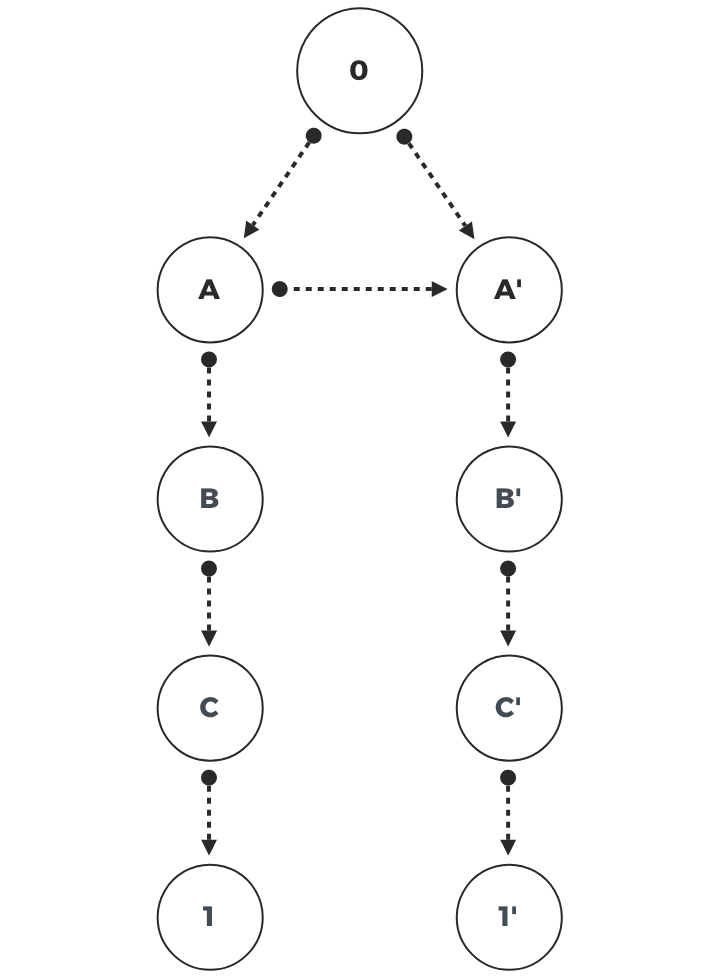
\includegraphics[width=\linewidth]{figures/Divergent_Heads.png}
  \caption{Divergent heads in a multi-writer Merkle-DAG }
  \label{fig:merkledag}
\end{figure}

A Merkle-Clock is a Merkle-DAG that represents a sequence of events. In other words, a Merkle-Clock is an append-only log \cite{sanjuanMerkleCRDTs2019}. When implemented on IPFS (or an equivalent network where content can be cryptographically addressed and fetched), Merkle-Clocks provide a number of benefits for data synchronization between replicas \cite[sec. 4.3]{sanjuanMerkleCRDTs2019}:

\begin{enumerate}
\item Broadcasting the Merkle-Clock requires broadcasting only the current root CID. The whole Clock is unambiguously identified by the CID of its root and its full DAG can be walked down from it as needed.
\item The immutable nature of a Merkle-DAG allows every replica to perform quick comparisons and fetch only those nodes that it does not already have.
\item Merkle-DAG nodes are self-verified and immune to corruption and tampering. They can be fetched from any source willing to provide them, trusted or not.
\item Identical nodes are de-duplicated by design: there can only be one unique representation for every event.
\end{enumerate}

On the downside, and as discussed above (Section \ref{sec:LogicalClocks}), a Merkle-Clock cannot order divergent heads (or roots). For example, in Figure \ref{fig:merkledag}, two replicas (top row, bottom row) are attempting to write (left to right) events to the same Merkle-Clock. After the first replica writes event A, the second writes event A' and properly links to A. At that point, the two replicas stop receiving events from one another. To a third replica that does continue to receive events, there would now be two independent heads, 1 and 1'. For the third replica, resolving these two logs of events may be costly (many updates happened since the last common node) or impossible (parts of the chain may not be available on the network). See Section  \ref{sec:EventualConsistency}.

In order to reduce the likelihood of divergent heads, all replicas should be perfectly connected and be able to fetch all events and linkages in the Merkle-Clock. On real networks with many often offline replicas (mobile and IoT devices, laptops, etc.), these conditions are rarely met. Based on these observations, using a single Merkle-Clock to synchronize replicas can be problematic.

% blocks the merkledag image from being rendered past here
\FloatBarrier

\subsection{Networking}

So far we have primarily discussed the mechanics of creating or linking content in a series of updates. Now we will overview some common networking tools for connecting distributed peers who aim to maintain replicas of a shared database. This could be any decentralized network of interacting entities (e.g., cloud servers, IoT devices, botnets, sensor networks, mobile apps, etc) collectively updating a shared state. IPFS contains a collection of protocols and systems to help address the networking needs required by different use-cases. That is to say no matter what type of device we are talking about --- be it a phone, desktop computer, browser, or Internet-enabled appliance --- it should be able to communicate with other devices. However, each of the networking approaches described below comes with strengths and weaknesses when used to synchronize data.

\subsubsection{Libp2p}

The libp2p project provides a robust protocol communication stack. IPFS and a growing list of other projects (Polkadot, Ethereum 2.0, Substrate, FileCoin, OpenBazzar, Keep, etc) are building on top of libp2p. Libp2p solves a number of challenges that are distinct to peer-to-peer (p2p) networks. A comprehensive coverage of networking issues in P2P systems is out of the scope for this paper, however, some core challenges that libp2p helps to address include network address translator \cite{srisureshIPNetworkAddress} (NAT) traversal, peer discovery and handshake protocols, and even encryption and transport security --- libp2p supports both un-encrypted (e.g. TCP, UDP) and encrypted protocols (e.g. TLS, Noise) --- among others. Libp2p uses the concept of a multiaddress to address peers on a network, which essentially models network addresses as arbitrary encapsulations of protocols \cite{multiformatsMultiaddr}. In addition to ``transport layer'' modules, libp2p provides several tools for sharing and/or disseminating data over a p2p network.

\subsubsection{Pubsub}

One of the most commonly used p2p distribution layers built on libp2p, is its Pubsub (or publish-subscribe) system. Pubsub is a standard messaging pattern where the publishers don't know who, if anyone, will subscribe to a given topic. \emph{Publishers} send messages on a given topic or category, and \emph{Subscribers} receive only messages on a give topic to which they are subscribed. Libp2p's pubsub module can be configured to utilize a \emph{floodsub} protocol --- which floods the network with messages, and peers are required to ignore messages they are not interested in --- or \emph{gossipsub} --- which is a proximity-aware epidemic pubsub, where peers communicate with proximal peers, and messages can be routed more efficiently. In those implementations, there is a benefit to using pubsub in that no direct connection between publishers and subscribers is required.

Another benefit to using pubsub is the ability to publish topical sequences of updates to multiple recipients. Like libp2p, encryption is a separate concern and often added in steps prior to data transmission. However, like libp2p, pubsub doesn't offer any simple solutions for transferring encryption keys (beyond public keys), synchronizing datasets across peers (i.e. they aren't databases), or enforcing any measures for access control (e.g. anyone subscribed to a topic can also author updates on that topic). To solve some of those challenges, some systems introduce message echoing and other partial solutions. However, it makes more sense to use pubsub and libp2p as \emph{building blocks} in systems that can effectively solve these issues, by choosing multi-modal communication strategies or leveraging tools such as deferred routing (e.g. inboxing) for greater tolerance of missed messages.

\subsubsection{IPNS}

Pubsub and libp2p have so far only dealt with \emph{push-based} transfer of data, but IPFS also offers a useful technology for hosting \emph{pull/request} based data endpoints called, IPNS. IPNS aims to address the challenge of mutable data within IPFS. IPNS relies on a global namespace (shared by participating IPFS peers) based on Public Key Infrastructure. By using IPNS, a content creator generates a new address in the global namespace and points that address to an endpoint (e.g. a CID). Using their private key, a content creator can update what static route the IPNS address refers to. IPNS isn't only useful for creating static addresses that can point to content addresses, IPNS is compatible with a naming system external from IPFS, such as DNS, onion, or bit addresses. However, many use-cases that require highly mutable data, require rapid availability of updates, or want flexible multi-party access control may not yet be suitable for IPNS. Taken together, libp2p, pubsub, IPNS, and IPFS more generally provide a useful toolkit for building robust abstractions to deliver fast, scalable, data synchronization in the decentralized network. 

\subsection{Data Access \& Control}

\subsubsection{Identity}

IPFS is an implementation of public key infrastructure, where every node on the IPFS network has a key-pair. In addition to using the key-pair for secure communication between nodes, IPFS also uses the key-pair as the basis for identity. Specifically, when a new IPFS node is created, a new key-pair is generated, and then the public key is transformed into the nodes Peer ID. 

\subsubsection{Agent-centric security}

Agent-centric security refers to the maintenance of data integrity without leveraging a central or blockchain-based consensus.
The general approach is just to let the reader enforce permissions and perform validations, not the writer or some central authority.
Agent-centric security is possible if the reader can reference local-only, tamper-free code or if the state can be used to determine whether a given operation (e.g. delete data) is permitted.
Many decentralized networks like Secure Scuttlebutt \cite{securescuttlebuttScuttlebuttProtocolGuide} and Holochain \cite{ericharris-braunHolochainScalableAgentcentric2018} make use of agent-centric security.
Each of these systems leverage cryptographic signatures to validate peer identities and messages.

\subsubsection{Access control}

All file-systems and databases have some notion of ``access control''. Many make use of an access-control list (ACL), which is a list of permissions attached to an object or group of objects \cite{shireyInternetSecurityGlossary2007}. An ACL determines which users or processes can access an object and whether a particular user or process with access can modify or delete the object (see Figure \ref{tbl:ACL}). 

\begin{table}
\caption{Example Access Control List.}
    \centering
    \begin{tabular} [t]{l>{\centering}p{0.15\linewidth}>{\centering}p{0.15\linewidth}>{\centering}p{0.15\linewidth}>{\centering\arraybackslash}p{0.15\linewidth}}
\toprule
&Create&Delete&Edit&Read\\
\midrule
Jane&-&-&-&\checkmark\\
John&\checkmark&\checkmark&\checkmark&\checkmark\\
Mary&-&-&\checkmark&\checkmark\\
\bottomrule
    \end{tabular}
    \label{tbl:ACL}
\end{table}

Using ACLs in systems where identity is derived from various configurations of public-key infrastructure has been around for some time \cite{herzbergAccessControlMeets2000}. Still, many existing database and communication protocols built on IPFS to date lack support for an ACL or only have primitive ACL support. Where ACLs are missing, many systems use cryptographic primitives like signature schemes or enable encryption without any role-based configuration. Even more, many systems deploy an all-or-none security model, where those with access to a database have complete access, including write capabilities. ACLs should be mutable over time and permission to modify an ACL should also be recorded in an ACL.

Event-driven systems (e.g., event sourcing) often make use of ACLs with some distinct properties. The ACL of an event-driven system is usually a list of access rules built from a series of events. For example, the two events, ``grant Bob write access'' and ``revoke read access from Alice'' would together result in a final ACL state where, Bob has read and write access, but Alice does not (Section  \ref{sec:ViewsProjections}).

\section{The Threads protocol}\label{sec:ThreadsProtocol}

We propose Threads, a protocol and decentralized database that runs on IPFS meant to help decouple apps from user-data. Inspired by Event Sourcing, CQRS, and Redux, Threads is a protocol for creating and synchronizing state across collaborating peers/replicas on a network. Threads offer a multi-layered encryption and data access architecture that enables datasets with independent roles for writing, reading, and following changes. By extending on the multiaddress addressing scheme, Threads differs from previous solutions by allowing PULL based replica synchronization in addition to PUSH based synchronization that is common in distributed protocols. The flexible event-based structure enables client applications to create advanced applications states, including materialized views, and custom CRDTs.

Threads are topic-based collections of single-writer logs. Taken together, these logs represent the current ``state'' of an object or dataset. The basic units of Threads, namely Logs and Events, provide a framework for users to create, store, and transmit data in a P2P distributed network. By structuring the underlying architecture in specific ways, this framework can be deployed to solve many of the problems discussed above.

\subsection{Event Logs}

In multi-writer systems, conflicts arise as disparate peers end up producing disconnected state changes, or changes that end up out of sync. In order to proceed, there must be some way to deal with these conflicts. In some cases (e.g, \texttt{ipfs-log} \cite{markroberthendersonOrbitDBFieldManual2019}), a Merkle-Clock can be used to induce ordering. This approach cannot achieve a total order of events without implementing a data-layer conflict resolution strategy \cite{sanjuanMerkleCRDTs2019}:

\begin{quote}
A total order can be useful \dots and could be obtained, for example, by considering concurrent events to be equal. Similarly, a strict total order could be built by sorting concurrent events by the CID or their nodes or by any other arbitrary user-defined strategy based on additional information attached to the clock nodes (data-layer conflict resolution).
\end{quote}

Solutions such as \texttt{ipfs-log} include a built-in CRDT to manage conflicts not resolved by the Merkle-Clock. This approach works for many cases, but the use of a deterministic resolution strategy can be insufficient in cases with complicated data structures or complicated network topologies. A git merge highlights one such example, in which a predetermined merge strategy can be used, but is not often the best choice in practice. Furthermore, a multi-writer log using a linked data format (e.g., a Merkle-Dag) in imperfect networking or storage environments can lead to suboptimal states where it may be exceedingly costly (networking, storage, and computation) to regain consistency.

A promising approach is one that can leverage the benefits of both a Merkle-Clock for events from any one peer and a less constrained ordering mechanism to combine events from all peers. In this more ideal setup, developers can more freely institute their own CRDTs or domain-specific conflict resolution strategies. Additionally, it more naturally supports use-cases where all peers contributing to a dataset may not be interested in following or replicating the events of all other peers. 

\subsubsection{Single-writer Event Logs}

% [!b] indicates that it will try to be on the bottom of the page
\begin{figure}[!t]
  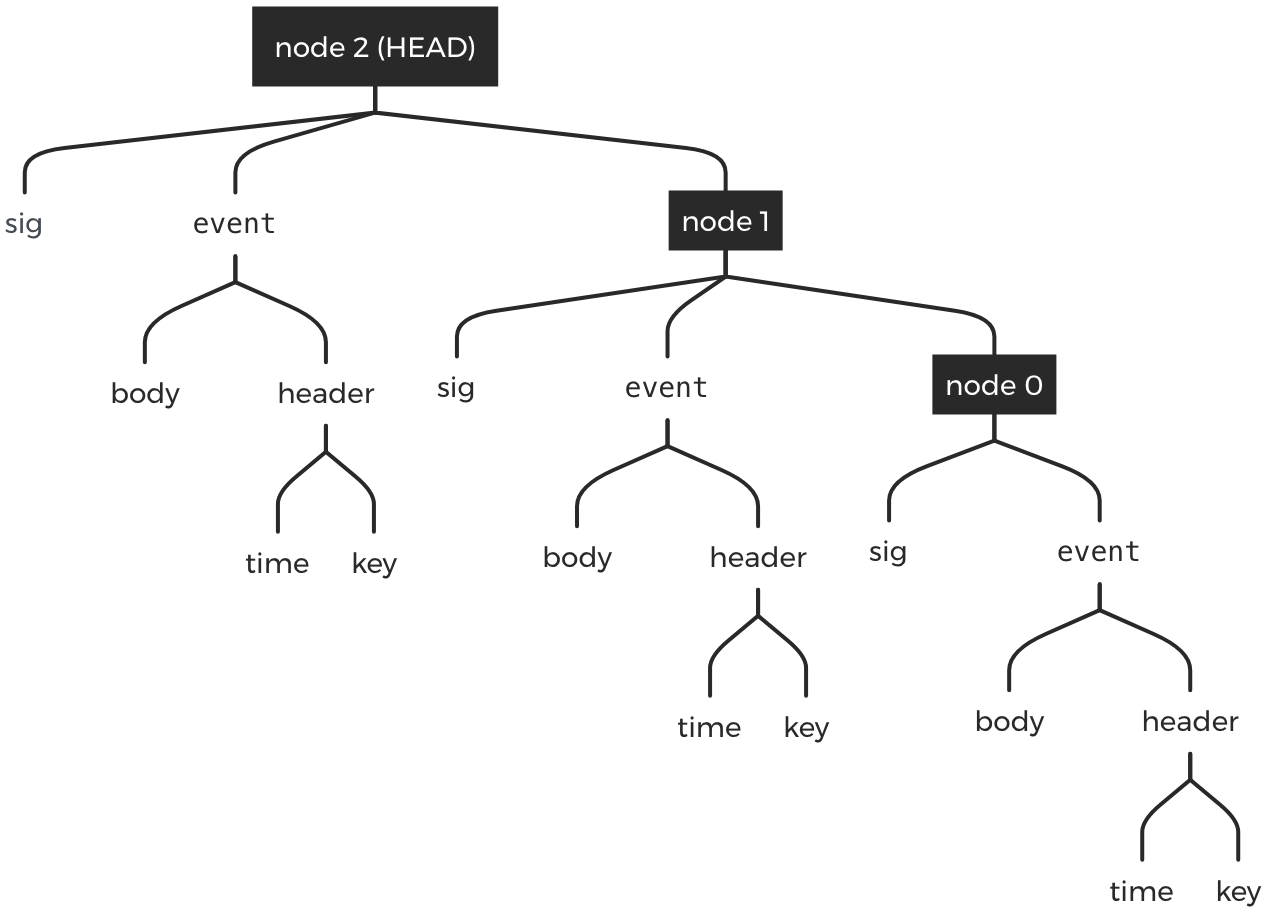
\includegraphics[width=\linewidth]{figures/Event_Log.png}
  \caption{A single-writer Merkle-Clock (Event Log).}
  \label{fig:EventLog}
\end{figure}

Our solution to dealing with log conflicts (i.e., divergent Merkle-Clocks) is to institute a \emph{single-writer rule}: A Log can only be updated by a single replica or \emph{identity}. An Event Log is then a \emph{single-writer Merkle-Clock} that can be totally ordered (Figure \ref{fig:EventLog}). \emph{Separate} Event Logs can be composed into advanced structures, including CRDTs \cite{enesSingleWriterPrincipleCRDT2017}.

This presents a novel take on multi-writer systems \cite{enesSingleWriterPrincipleCRDT2017}, such that conflict resolution is deferred to a point at which a decision is actually \emph{required}. This means that imperfect information may be supplemented along the way (i.e., at a later time), without causing conflicts in the mean time. It also means that applications can choose conflict resolution strategies specific to the task at hand. For example, if using a downstream CRDT, ordering is actually irrelevant, and can be ignored completely. Alternatively, an additional clock may be required to ensure consistent ordering, such as a vector or Bloom clock (see Section \ref{sec:LogicalClocks}). Finally, even manual merge-type strategies are possible if this is the desired conflict resolution strategy.

For any given Log, Events are authored by a single IPFS Peer, or \emph{Writer}.

\begin{definition}
(Writer). The single IPFS Peer capable of writing to an Event Log.
\end{definition}

This single-writer setup is a core feature of Logs, and provides properties unique to the Threads protocol. For clarity, we can similarly define a \emph{Reader} as any other Peer capable of reading a Log.

\begin{definition}
(Reader). Any Peer capable of reading a Log. Practically speaking, this means any Peer with the Log's Read Key (Section  \ref{sec:KeysEncryption}).
\end{definition}

As seen above in Section \ref{sec:merkleclocks}, a Merkle-Clock is simply a Merkle-DAG of \emph{Events}:

\begin{definition}
 (Event). A single node in a Merkle-Clock, stored on IPFS.
\end{definition}

% blocks the EventLog image from being rendered past here
\FloatBarrier

\begin{example*}[!b]
\centering
\begin{minipage}{0.7\textwidth}
\begin{lstlisting}[language=json,firstnumber=1]
# Log multiaddress
 /ipel/12D3KooWC2zyCVron7AA34N6oKNtaXaZB51feG9rBkr7QbCcW8ab

# Encapsulated multiaddress
 /ip4/127.0.0.1/tcp/1234/p2p/12D..dwaA6Qe/ipel/12D..bCcW8ab

# Address book
[
  /p2p/12D..dwaA6Qe/ipel/12D..bCcW8ab,
  /p2p/12D..dJT6nXY/ipel/12D..bCcW8ab # Follower
]
\end{lstlisting}
\end{minipage}
  \caption{The Log Multiaddress.}
  \label{ex:Multiaddress}
\end{example*}

\subsubsection{Multi-addressed Event Logs}

Together with a cryptographic signature, an Event is written to a log with an additional node (see Figure \ref{fig:EventLog}) enabling log verification by readers (Section \ref{sec:KeysEncryption}).

At a minimum, a node must link to its most immediate ancestor. However, links to older ancestors are often included as well to improve concurrency during traversal and verification \cite{meyerBamboo2019}.

As shown \ref{appx:EventNode}, an Event's actual content, or body, is contained in a separate node. This allows Events to carry any arbitrary node structure, from complex directories to raw bytes.

Much like IPFS Peers, Logs are identified on the network with addresses, or more specifically, with multiaddresses\cite{multiformatsMultiaddr}. Here we introduce IPEL, or Interplanetary Event Log, as a new protocol tag to be used when composing Log multiaddresses. To reach a Log via it's IPEL multiaddress, it must be encapsulated in an IPFS Peer multiaddress (see Example \ref{ex:Multiaddress}).

In practice, to reach a Log via it's IPEL multiaddress, it must be encapsulated in an IPFS Peer multiaddress (Example \ref{ex:Multiaddress}).

Unlike peer multiaddresses, Log addresses are not stored in the global IPFS distributed hash table \cite{benetIPFSContentAddressed2014} (DHT). Instead, they are collected from Log Events. This is in contrast to mutable data via IPNS for example, which requires querying the network (DHT) for updates. Instead, updates are requested directly from the (presumably trusted) peers that produced them, resulting in a hybrid of content-addressed Events arranged over a data-feed\footnote{This is similar to the append-only message feeds used in Secure Scuttlebutt’s global gossip network \cite{securescuttlebuttScuttlebuttProtocolGuide}} like topology. Log addresses are recorded in an address book, similar to IPFS Peer address book (Example \ref{ex:KeyBook}).

Addresses can expire by specifying a time-to-live (TTL) value when adding or updating them in the address book, which allows for unresponsive addresses to eventually be removed.

Modern, real-world networks consist of many mobile or otherwise sparsely connected computers (Peers). Therefore, datasets distributed across such networks can be thought of as highly partitioned. To ensure updates are available between mostly offline or otherwise disconnected Peers (like mobile devices), Textile Logs are designed with a built-in replication or follower mechanism.

\begin{definition} (Follower). Log Writers can designate other IPFS Peers to ``follow'' a Log, potentially replicating and/or republishing Events. A Follower is capable of receiving Log updates and traversing linkages via the Follow Key (Section  \ref{sec:KeysEncryption}), but is not able to read the Log's contents. Followers should be server-based --- i.e., always online and behind a public IP address.\end{definition}

Followers are represented as additional addresses, meaning that a Log address book may contain \emph{multiple} multiaddresses for a single Log (Example \ref{ex:Multiaddress}).

In practice, Writers are solely responsible for announcing their Log's addresses. This ensures a conflict-free address list without additional complexity. Some Followers may be in the business of replicating Logs (Section  \ref{sec:Bots}), in which case Writers will announce the additional Log address to Readers. This allows them to \emph{pull} (or subscribe to push-based) Events from the Follower's Log address when the Writer is offline or unreachable (Figure \ref{fig:Pulling}).

\subsubsection{Keys \& Encryption} \label{sec:KeysEncryption}

\begin{figure*}[!t]
\centering
\begin{minipage}{0.6\textwidth}
  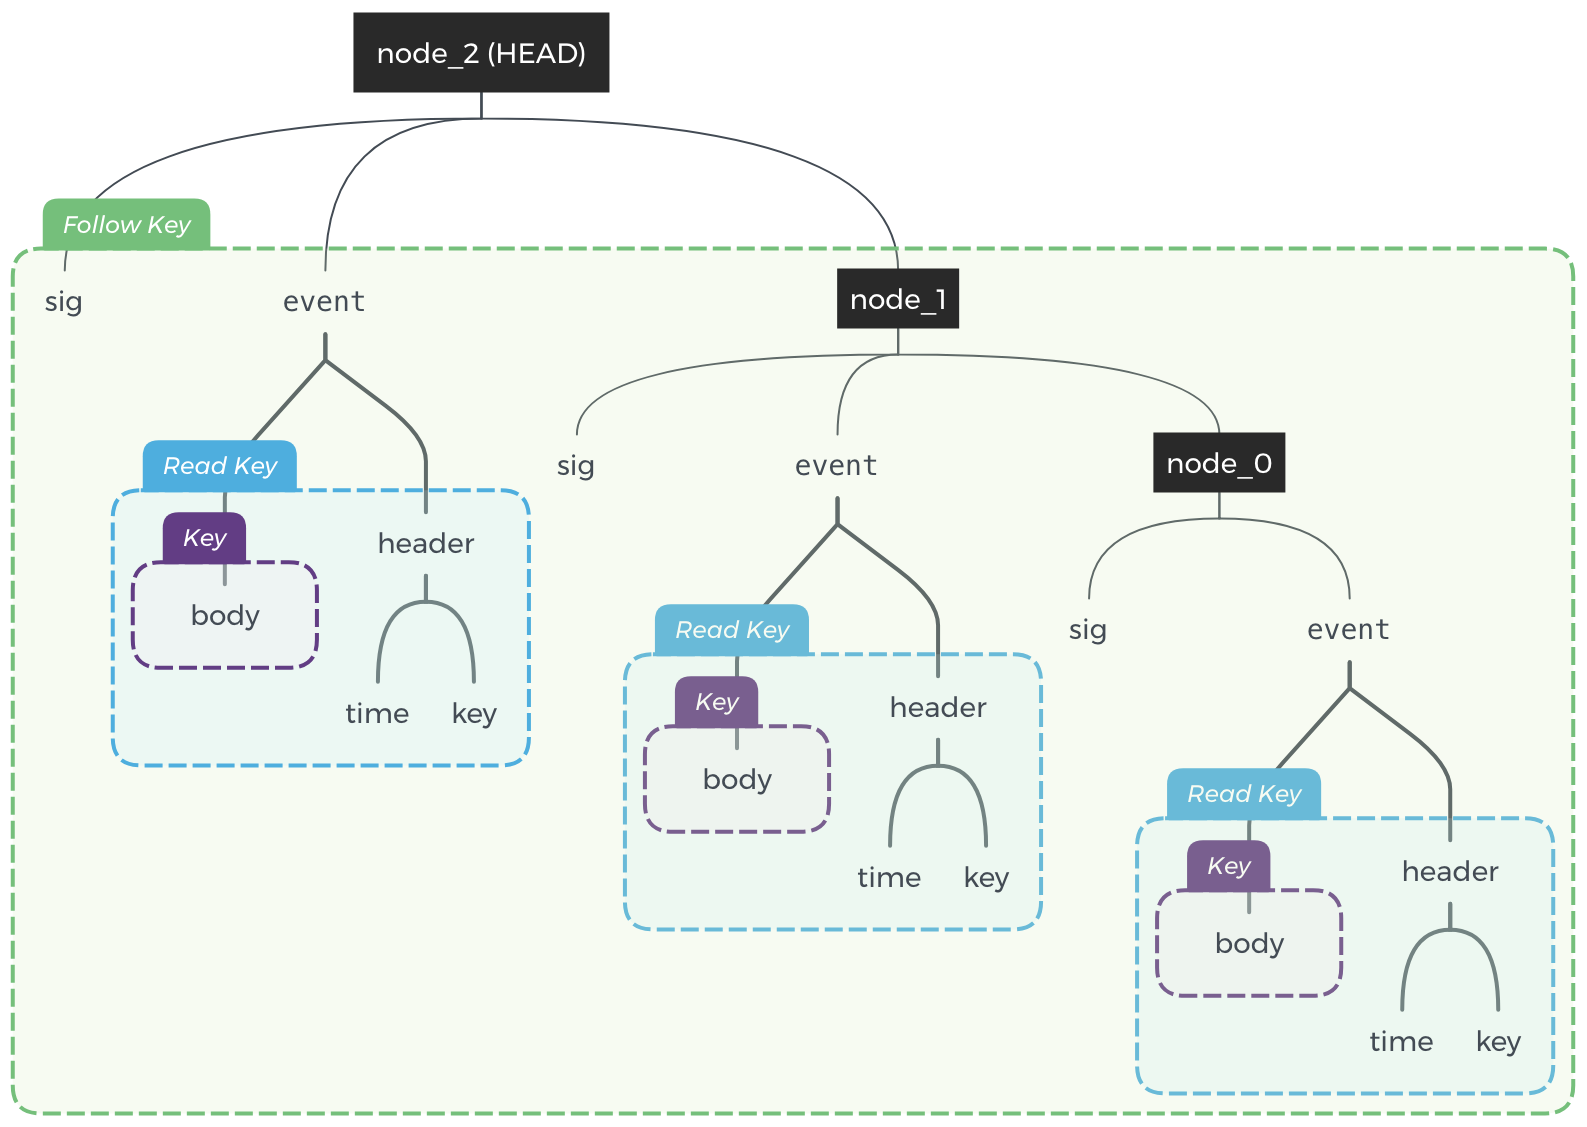
\includegraphics[width=\linewidth]{figures/Event_Log_With_Encryption.png}
  \caption{The three layers of Log Event encryption.}
  \label{fig:LogEncryption}
  \end{minipage}
\end{figure*}

\begin{example}[!b]
\begin{lstlisting}
type AddrBook interface {
   AddAddr(thread.ID, peer.ID, ma.Multiaddr, time.Duration)
   AddAddrs(thread.ID, peer.ID, []ma.Multiaddr, time.Duration)
   SetAddr(thread.ID, peer.ID, ma.Multiaddr, time.Duration)
   SetAddrs(thread.ID, peer.ID, []ma.Multiaddr, time.Duration)
   UpdateAddrs(t thread.ID, id peer.ID, oldTTL time.Duration, newTTL time.Duration)
   Addrs(thread.ID, peer.ID) []ma.Multiaddr
   ClearAddrs(thread.ID, peer.ID)
}
type KeyBook interface {
   PubKey(thread.ID, peer.ID) ic.PubKey
   AddPubKey(thread.ID, peer.ID, ic.PubKey) error
   PrivKey(thread.ID, peer.ID) ic.PrivKey
   AddPrivKey(thread.ID, peer.ID, ic.PrivKey) error
   ReadKey(thread.ID, peer.ID) []byte
   AddReadKey(thread.ID, peer.ID, []byte) error
   FollowKey(thread.ID, peer.ID) []byte
   AddFollowKey(thread.ID, peer.ID, []byte) error
}
\end{lstlisting}
\caption{The AddrBook interface for storing log addresses and the KeyBook interface for storing log keys.}
\label{ex:KeyBook}
\end{example} 


Textile Logs are designed to be shared, composed, and layered into datasets (Figure \ref{fig:LogEncryption}). Therefore, Logs are encrypted by default in a manner that enables access control (Section  \ref{sec:AccessControl}) and the Follower mechanism discussed in the previous section.

\begin{definition}
(Identity Key). Every Log requires an asymmetric key-pair that determines ownership and identity. The private key is used to sign each Event added to the Log, so down-stream processes can verify the Log's authenticity. Like IPFS peers, the public key of the Log is used as an identifier (Log ID).
\end{definition}

The body, or content of an event, is encrypted by a \emph{Content Key}. Content Keys are generated per-content and never reused. The Content Key is distributed directly in the header of the Event Block. We define the Content Key as follows,

\begin{definition}
(Content Key). The Content Key is a variable-format key used to encrypt the body (content) of an event. This key can be symmetric, asymmetric, or possibly non-existent in cases where encryption is not needed. One of two common encryption choices will typically be used per event, 
\begin{enumerate}
\item When broadcasting events to many possible recipients, a single-use symmetric key is generated per unique content body.
\item When sending events to specific recipients, the recipient's public key can be used to restrict access from all others\footnote{Much like private messages in Secure Scuttlebutt (\url{https://www.scuttlebutt.nz/concepts/private-message})}.
\end{enumerate}
\end{definition}

If a single-use symmetric key is used for the Content Key, it is necessary to distribute each new key to users by including it in the header of the Event Block. Therefore, the Event Block itself is further encrypted using a \emph{Read} key. The Read Key is not distributed within the Log itself but is distributed to any peers to grant them access to the content of the Log. 

\begin{definition}
 (Read Key). The Read Key is a symmetric key created by the Log owner and used to encrypt the Content Key in each event.
\end{definition}

Finally, the encrypted Event Block, its signature, and the IPLD linkage(s) from an Event to its antecedents are encrypted together using a Follow Key. Follow Keys allow Logs to be \emph{followed} by peers on the network who do not have access to any content within the event, and can only see signatures and linkage(s) between Events.

\begin{definition}
(Follow Key). The Follow Key is a symmetric key created by the Log owner and used to encrypt the entire event payload before adding the event to the Log.
\end{definition}

Much like the Log address book, Log keys are stored in a key book (Example \ref{ex:KeyBook}).

\subsection{Threads}

In Textile, the \emph{interface} to Logs is managed as a Thread. As mentioned previously, a Thread is a collection of Logs on a given topic. Threads are an event-sourced, distributed database, and can be used to maintain a single, collaboratively edited, watched, or hosted dataset across multiple Peers. Threads provide the mechanism to combine multiple Logs from individual authors into singular shared states through the use of either cross-Log sequencing (e.g. using a Bloom Clock, Merkle-Clock, or Hybrid Logical Clock \cite{kulkarniLogicalPhysicalClocks2014}) or a CRDT (Section \ref{sec:CRDTs}).

\subsubsection{Identity}

A unique Thread IDentity (TID) is used to group together Logs which compose a single dataset and as a topic identifier within Pub/Sub-based synchronization. TIDs are defined with the format shown Figure \ref{fig:ThreadID}.

\begin{figure*}[th]
\centering
\caption{Components of a Thread Identity.}
\par\vspace{.9\baselineskip}\leavevmode%
\par{Thread ID = 0x62\quad}\ubar{0x01}{Version}\quad0x55\quad\ubar{0x539bc1dc03ee8cb5d478e41cc8a4546e}{Random Number} 
\par\vspace{-.6\baselineskip}\leavevmode%
\phantom{Thread ID = }\phubar{0x62}{Multibase}%
  \phantom{\quad0x01\quad}\phubar{0x55}{Variant} \phantom{\quad0x539bc1dc03ee8cb5d478e41cc8a4546}
\label{fig:ThreadID}
\end{figure*}

TIDs share some similarities with UUIDs \cite{leachUniversallyUniqueIDentifier2005} (version and variant) and IPFS-based CIDs and are multibase encoded\footnote{\url{https://github.com/multiformats/multibase}} for maximum forward-compatibility.

\begin{definition}
(Multibase Prefix). The encoding type used by the multibase encoder. 1 byte.
\end{definition}

Base32 encoding is used by default. However, any multibase-supported string encoding may be used.

\begin{definition}
(Version). ID format version. 8 bytes max. This allows future version to be backwards-compatible.
\end{definition}

\begin{definition}
(Variant). Used to specify thread-level expectations, like access-control. 8 bytes max. See section 3.2.2 for more about variants.
\end{definition}

\begin{definition}
(Random Number). A random number of a user-specified length. 16 bytes or more  (see Example \ref{ex:Identity}).
\end{definition}

\subsubsection{Variants}\label{sec:variants}

Certain ID \emph{variants} may be more appropriate than the others in specific use cases. For example, Textile provides an \emph{access-controlled} Thread variant, which supports various collaborative structures --- e.g., social media feeds, shared documents, blogs, photo albums, etc.

\begin{definition}
(Raw). This variant declares that consumers are not expected to make additional assumptions. This is the default variant (See Example \ref{ex:Identity}a).
\end{definition}

\begin{definition}
(Access-Controlled): This variant declares that consumers should assume an access control list is composable from Log Events. The ACL represents a permissions rule set that must be applied when reading data (Section  \ref{sec:AccessControl} and Example \ref{ex:Identity}b).
\end{definition}

\begin{example}[hb]
\centering
\begin{minipage}{0.6\textwidth}
\begin{lstlisting}[language=json,firstnumber=1]
# (a) Raw identity. V1, 128 bit
bafkxd5bjgi6k4zivuoyxo4ua4mzyy

# (b) ACL enabled identity. V1, 256 bit.
bafyoiobghzefwlidfrwkqmzz2ka66zgmdmgeobw2mimktr5jivsavya
\end{lstlisting}
\end{minipage}
  \caption{Identity variants.}
  \label{ex:Identity}
\end{example}

\subsubsection{Log Synchronization} \label{sec:LogSync}

Log Writers, Readers, and Followers synchronize the state of their Logs by sending and receiving Events. Inspired by Git\footnote{\url{https://git-scm.com/}}, a reference to the latest Event in a Log is referred to as the \emph{Head} (or sometimes the \emph{root}). When a new Event is received, Readers and Followers simply advance their Head reference for the given Log\footnote{This is similar to how a system such as OrbitDB [MISSING] works, except we are tracking \emph{multiple} Heads (one per Log), rather than a single Head.}.

Regardless of the network protocol, Events are transported between Peers in a standardized \emph{Event Envelope}:

\begin{definition}
(Event Envelope). An over-the-wire message containing an Event and the sender's signature of the Event.
\end{definition}

A new Thread is created by generating a TID and Log. The Log's creator is the Writer, meaning it has possession of the Log's Identity, Read, and Follow Keys. All of these keys are needed to compose Events. At this point, the Thread only exists on the Writer's machine. Whether for collaboration, reading, or following, the process of sharing a Thread with other Peers starts by authoring a special Event called an \emph{Invite}, which contains a set of keys from all of the Thread's Logs, called a \emph{Key Set}.

\begin{definition}
(Invite). An Event containing a mapping of Log IDs to Key Sets, which can be used to join a Thread. Threads backed by an access control list (Section  \ref{sec:AccessControl}) will also include the current ACL for the Thread in an Invite. This enables Peers to invite others to only read or follow a Thread, instead of becoming a full-on collaborator, i.e., a new Log Writer.
\end{definition}

\begin{definition}
(Key Set). A set of keys for a Log. Depending on the context, a Key Set may contain the Follow and Read Key, or just the Follow Key. Encrypted with the recipient's public key.
\end{definition}

The Invite is authored in the sender's Log. Because the recipient does not yet have this Log's Key Set, the Event is encrypted with the recipient's public key. If the recipient accepts the Invite, they will author another special Event called a \emph{Join} in a new Log of their own.

\begin{definition}
(Join). An Event containing an invitee's new Log ID and Key Set, encrypted with the Key Set of the \emph{inviting Peer's Log}.
\end{definition}

For a Join to be successful, all Log Writers must receive a copy of the new Key Set so they can properly handle future Events in the new Log. Instead of encrypting a Join with the public key of each existing Writer, we can encrypt a single Join with the Key Set of the inviting Peer's Log, which the other Writers also have.

Once a Peer has accepted an Invite, it will receive new Events from Log Writers.
In cases where the invitee becomes a collaborator (i.e., a Writer) it is also responsible for sending its own Events out to the network.

\paragraph{Sending}

Sending is performed in multiple phases because, invariably, some Thread participants will be offline or unresponsive. 

\begin{enumerate}
\item New Events are pushed\footnote{Here push means ``send to multiaddress(es)'', which may designate different protocols, e.g., p2p, HTTP, Bluetooth, etc.} directly to the Thread's other Log Writers.
\item New Events are pushed directly to the target Log's Follower(s), who may not maintain their own Log.
\item New Events are published over Libp2p's gossip-based Pub/Sub infrastructure using TID as a topic, which provides potentially unknown Readers or Followers with an opportunity to consume Events in real-time.
\end{enumerate}

Step 2 above allows for \emph{additional} push mechanisms, as followers with public IP addresses become relays:

\begin{enumerate}
\item New Events may be pushed directly to web-based participants over a WebSocket.
\item New Events may be pushed to the Thread's other Log Writers via federated notification services like Apple Push Notification Service (APNS), Google Cloud Messaging (GCM), Firebase Cloud Messaging (FCM), and/or Windows Notification Service (WNS).
\item New Events may trigger web-hooks\footnote{\url{https://en.wikipedia.org/wiki/Webhook}}, which could enable many complex (e.g., IFTTT\footnote{\url{https://ifttt.com}}) workflows.
\end{enumerate}

\paragraph{Receiving}

There are multiple paths to receiving new Events, that together, maximize connectivity between Peers who are often offline or unreachable.

\begin{enumerate}
\item Log Writers can receive Events directly from the author.
\item Events can be pulled from replicating Followers via HTTP, libp2p, RSS, Atom, etc.
    a. In conjunction with push over WebSockets (seen in Step 2 of the additional push mechanisms above), this method provides web-based Readers and Followers with a reliable mechanism for receiving Log Events (Figure \ref{fig:Pulling}).
\item Writers and readers can receive new Events via a Pub/Sub subscription at the TID.
\end{enumerate}

\begin{figure}
  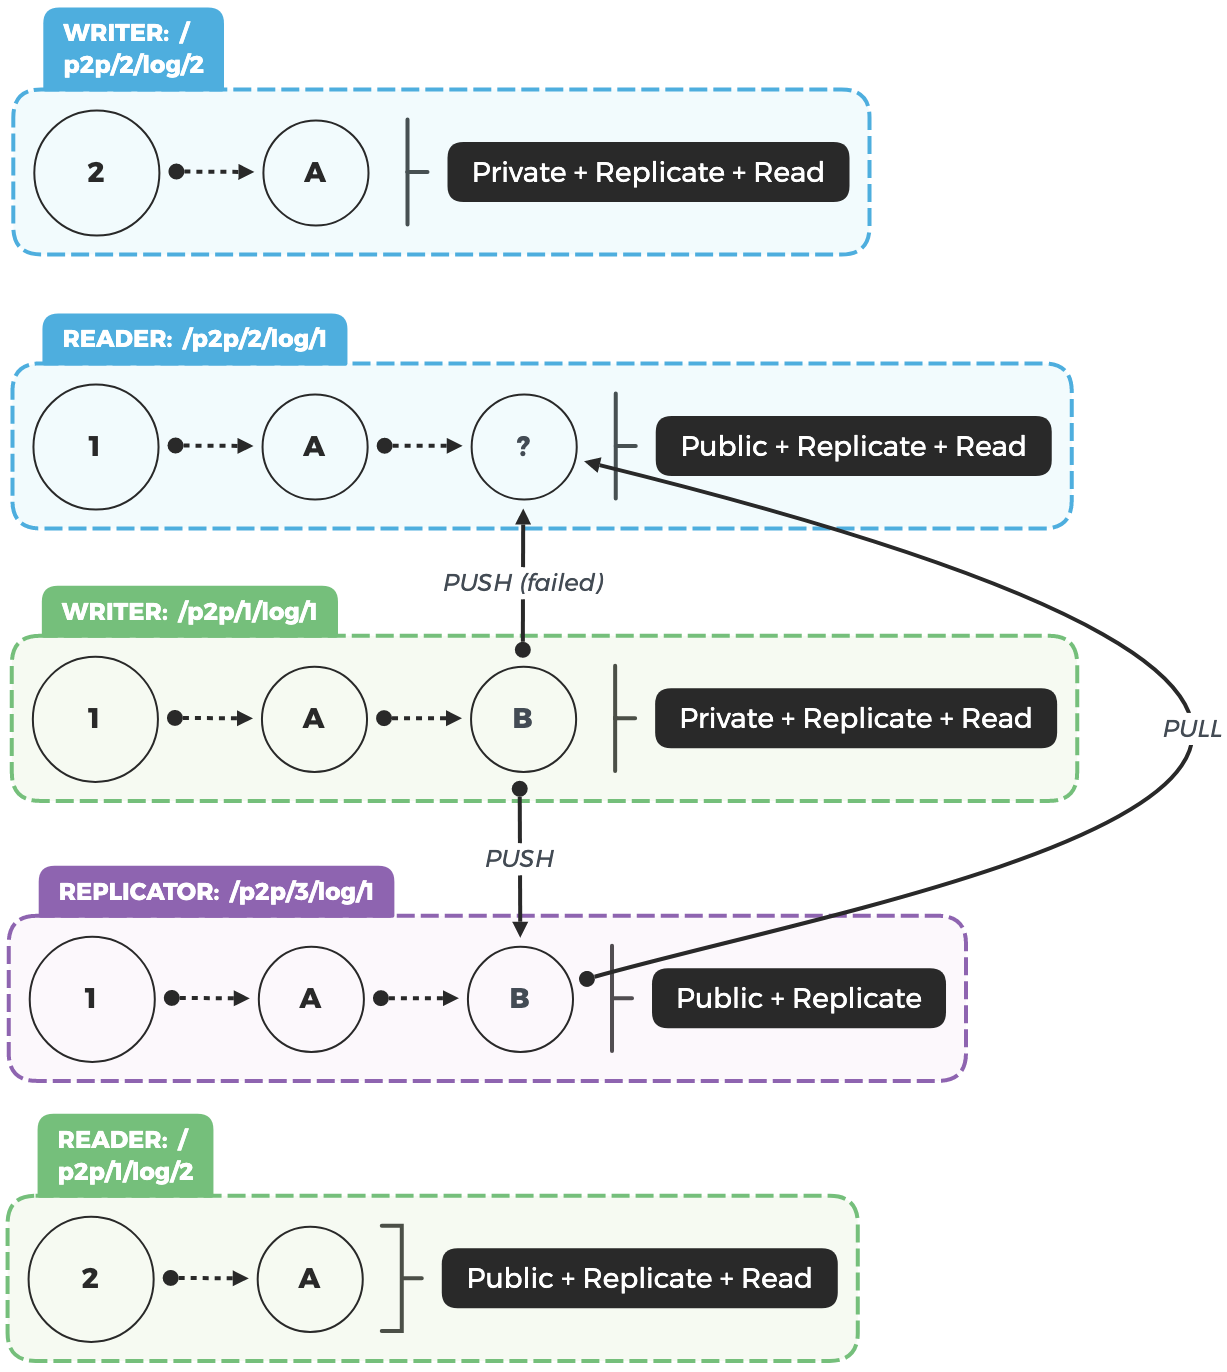
\includegraphics[width=\linewidth]{figures/Pulling.png}
  \caption{A pull-based request from a Follower.}
  \label{fig:Pulling}
\end{figure}

\subsubsection{Log Replication}

The notion of the Follow Key (Section  \ref{sec:KeysEncryption}) makes duplicating all Log Events trivial. This allows any Peer in the network to be granted the responsibility of replicating data from another Peer without having read access to the data contained within the Log entries. This type of Log replication can act as a data backup mechanism. It can also be used to build services that react to Log Events, potentially pushing data to disparate, non-Textile systems, especially if the replication service is granted read access to the Log Events (Section  \ref{sec:LogSync}).

\section{Threads Internals}\label{sec:internals}

Previous sections have discussed the core features of the Textile Threads protocol. However, we have not yet discussed dealing with Log Events in practice. In this section, we provide a description of a Threads-compatible Event Store implementation. The Event Store outlined here takes advantage of ideas from several existing CQRS and ES systems (e.g., \cite{ereminReduxInspiredBackend2019}), as well as concepts and designs from Flux \cite{facebookFluxInDepthOverview2019}, Redux\footnote{Redux builds on concepts from CQRS and ES itself, and is arguably an implementation of the Flux application architecture.} \cite{reduxMotivation} and domain driven design \cite{evansDomaindrivenDesignTackling2004a} (DDD)\footnote{\url{https://dddcommunity.org}}. Following this discussion of Threads \emph{internals}, in Section \ref{sec:interfaces} we outline how it can be used to build intuitive developer-facing application programing interfaces (APIs) to make adopting and using Threads ``the right choice'' for a wide range of developers.

\subsection{Overview}

Application state management tools such as Redux provide opinionated frameworks for making state mutations \emph{predictable} by imposing certain restrictions on how and when updates can happen. If you take a look at the architecture of such an application, you'll notice several core similarities to CQRS and ES systems (see \cite{facebookFluxInDepthOverview2019} and/or \cite{abramovCaseFlux2015}). In both cases, the focus is on unidirectional data flows that build downstream views from atomic updates in the form of events (or actions).

\begin{figure}
  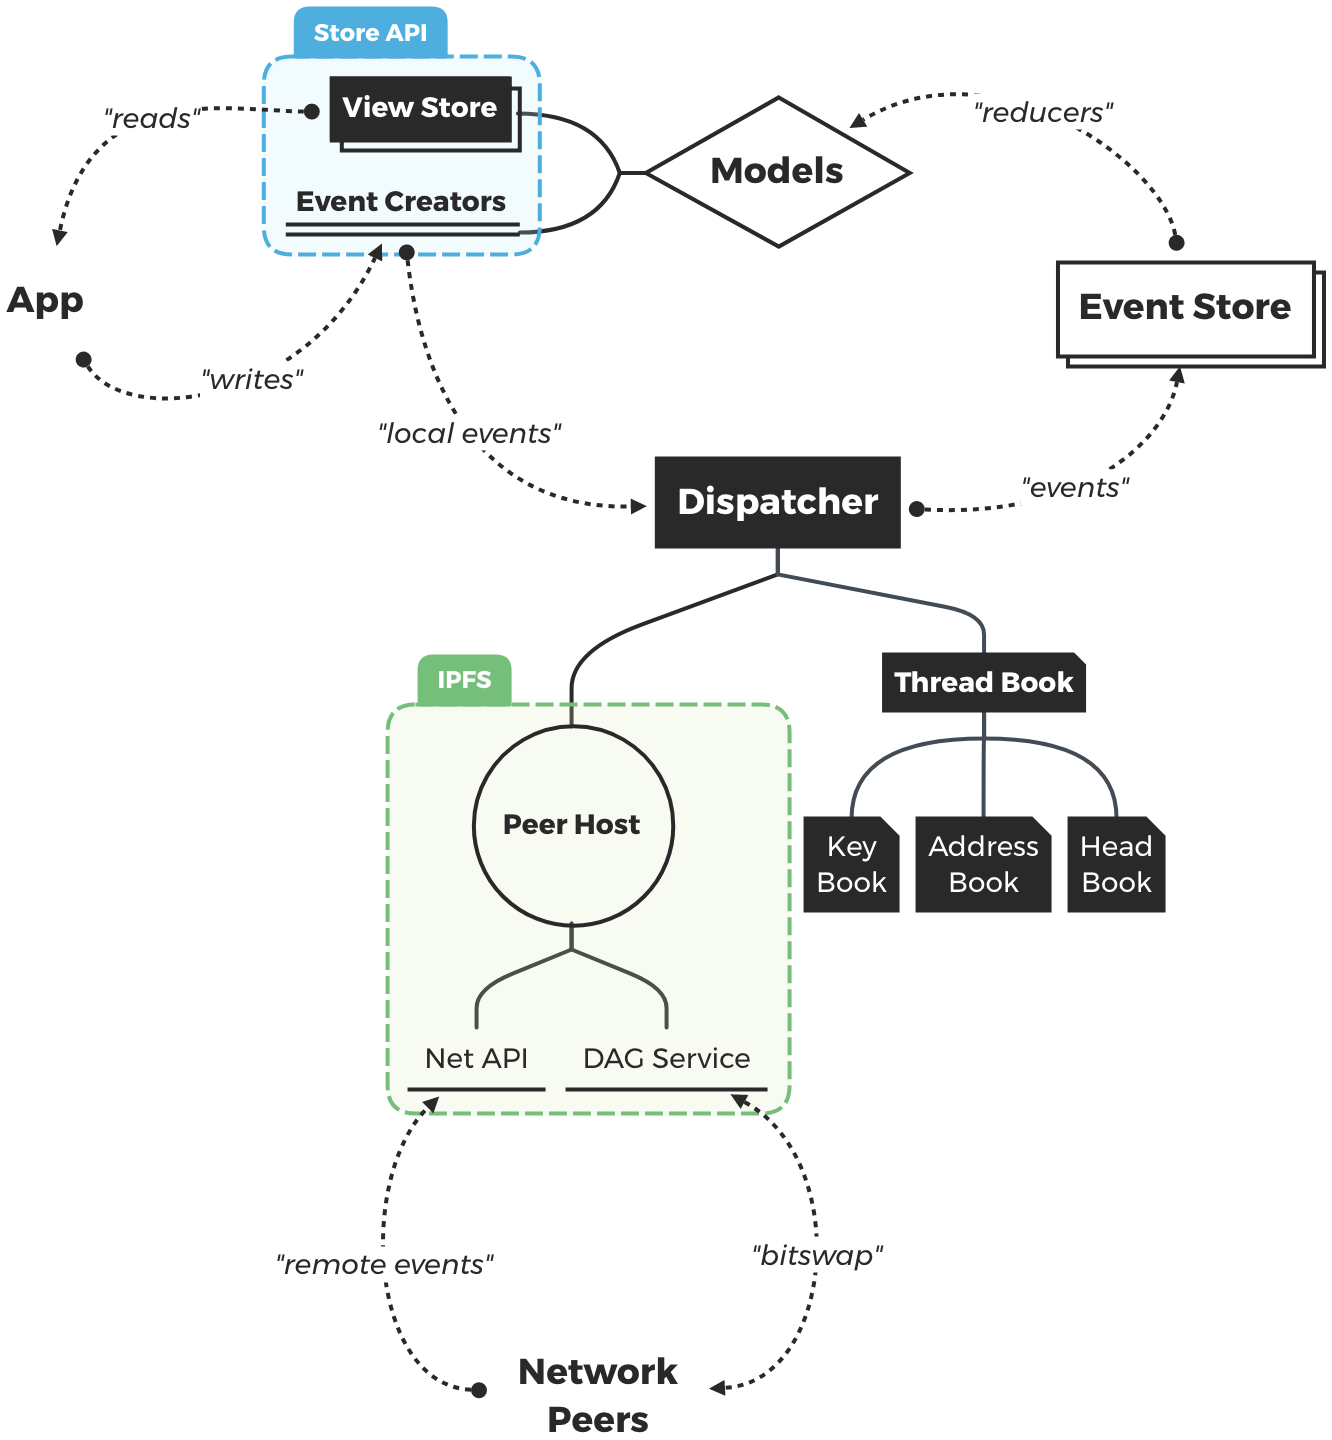
\includegraphics[width=\linewidth]{figures/Architecture.png}
  \caption{Architectural diagram for internal Event Store implementation.}
  \label{fig:Architecture}
\end{figure}

We adopt a similar flow in Threads (see Figure \ref{fig:Architecture}). Like any ES-based system, Threads are built on \emph{Events}. Events are similar to actions in a Flux-based system, and are used to produce \emph{predictable} updates to downstream state. Similarly to a DDD-based pattern, to add an Event to the internal Threads system, we use \emph{Event Creators}, which dispatch Events to the system via a singleton \emph{Dispatcher}. The Dispatcher then stores the derived Event in an \emph{Event Store}, and calls a set of registered \emph{Reducer} functions that mutate a (set of) downstream view \emph{Stores} defined by a corresponding set of view \emph{Models}, all within a single \emph{Transaction}. This unidirectional, transaction-based system, provides a flexible framework for building complex event-driven application logic.

\subsubsection{Events \& Creators}\label{sec:creators}

Like most CQRS + ES based systems, \emph{Events} are at the heart of Threads. Every update to local and shared (i.e., across peers) application state happens via Events (see also Section \ref{sec:cqrs}). Events are similar to actions in Redux, and are used to describe ``changes to an application state'' \cite{fowlerEventSourcing} (e.g., a photo was added, an item was added to a shopping cart, etc). Related, \emph{Event Creators} are used to send Events from a \emph{local application} to an internal Event Store. If built around a specific \emph{domain}, Creators provide bounded context that can be roughly compared to an aggregate root in DDD \cite{evansDomaindrivenDesignTackling2004a}.

\subsubsection{Dispatcher}\label{sec:dispatcher}

In order to actually persist and dispatch Events to downstream view Models, a \emph{Dispatcher} is used. As shown in Figure \ref{fig:Architecture}, the Dispatcher is at the center of the ES system. All Events must go through the singleton Dispatcher, whether these be from local Event Creators, or Network Peers. The Dispatcher is responsible for ensuring that incoming Events are persisted to the Event Store (the ``source of truth'' for the system), as well as dispatched to downstream view Models by way of a set of Reducer functions.

% \begin{definition}
%   (Dispatcher). A Dispatcher is used to both persist Events to the local Event Store, as well as broadcast Event payloads to registered Store Reducers. Only one Dispatcher per application is ever required.
% \end{definition}

\subsubsection{Transactions}\label{sec:transactions}

All Reducer function calls (and ``side effects'') due to a given Event happen within a single \emph{Transaction} \cite{haerderPrinciplesTransactionorientedDatabase1983}, in order to ensure consistently of both storage (Event Store) and Models. Transactions are similar to Redux \emph{Sagas}\footnote{\url{https://redux-saga.js.org/}} in terms of outcome, but with stronger consistency guarantees. Once an Event has been persisted in the internal Event Store, the Dispatcher is responsible for running a view Model's Reducer callback. In order to make this possible, Models must \emph{register} their Reducer with the Dispatcher.

% Events can also be \emph{batch dispatched}, which is the preferred way to dispatch multiple Events at a time. This works by grouping Events, and then running their Reducers in series. An example of where this is useful is when grouping externally derived \emph{Peer-Events}, which can be dispatched directly from the local Peer Host.

\subsubsection{View Models/Stores}\label{sec:views}

As in many CQRS-based systems, Events are dispatched on the write side, and are \emph{reacted to} on the read side. Reactions happen via Reducer fuctions, which cause updates to view Models, which in turn provide interfaces for queries and accessing persisted view \emph{Stores} (state). View Stores are then responsible for notifying downstream consumers (application logic) of changes to their state via a \emph{Broadcaster} (i.e., event emitter). They are similar in some respects to a Redux Store, though it is possible to have \emph{multiple} view Models/Stores as in the more general Flux pattern.

A view Model is generally defined by custom update logic (i.e., a Reducer), a (possibly ORM\footnote{Object-relational mapping}-based) view Store for persistence, an Event Bus (or Broadcaster) for notifying downstream consumers, and a set of query/\emph{Resolver} \cite{ereminReduxInspiredBackend2019} functions. In practice, a view Model may \emph{also} wrap the Event Creator application logic that is used to generate upstream Events. This provides an intuitive, singular access point to the \emph{local} system, while also leaving room for updates via \emph{external} peer-events. In practice, the Store is a lightweight interface that can be implemented by one of many database management systems (\ref{appx:DBMS}).

\subsubsection{External Events}\label{sec:external}

In addition to locally derived Events (i.e., from application logic and user interactions), Threads are designed so that Peers may collaborate in a given Thread via Events. Events generated by other, network peers are called Peer Events, and they enter the system via a Peer Host. The Peer Host is responsible for dealing with incoming Events (be they push or pull). These Events are no different from locally-derived Events, though in practice, the Peer Host is required to validate incoming Events before they are dispatched to the system via the Dispatcher.

% \begin{definition}
%   (Reducer). Reducers are ``pure'' (in the functional sense) functions\footnote{In practice they aren't really pure, because we are mutating (persistent) state here}, and are written to modify a Store's state based on incoming Actions.
% \end{definition}

% \begin{definition}
%   (Resolver). Resolvers are simply pre-defined query functions that exist on the Store instance (i.e., the Store's API). The interesting thing here is that these can similarly be defined around a domain to produce domain aggregates (in the DDD sense).
% \end{definition}

% \begin{definition}
%   (Store). Stores provide flexible APIs for persisting and accessing state. They are defined by a Reducer function for handling incoming Actions, and a set of query Resolver functions for handling queries. They are additionally responsible for notifying downstream consumers of updates to their state via a Broadcaster.
% \end{definition}

\section{Thread Interfaces}\label{sec:interfaces}

To make Threads as easy to adopt and use as possible, Textile has designed a developer facing API on top of the Threads internals that simplifies dealing with events and data, while still maintaining the power and flexibility of CQRS and ES. Developers should not have to learn a whole new set of terms and tools to take advantage of Textile's Threads capabilities. These simple, public-facing APIs will be comfortable to application developers looking to leverage highly-distributed systems that connect user-controlled data, with minimal configuration and maximum interoperability. Inspired by tools such as MondoDB\footnote{\url{http://www.mongodb.com}}, Parse\footnote{\url{https://parseplatform.org}}, and Realm\footnote{\url{https://realm.io}}, as well as the idea of bounded context and aggregate roots from DDD, we provide simple abstractions for performing distributed database operations as if they were local.

Indeed, the components of a Thread already provide several features that you would expect when operating on a dataset or table within a database: each Thread is defined by a unique ID, and provides facilities for access control and permissions, networking, and more. To illustrate how these underlying components can we combined to produce a simple API with minimal configuration and boilerplate, consider the following example, in which we provide pseudo-code for a hypothetical Photos application.

\subsection{Illustrative Example}\label{sec:example}

% For any application, the first step would be to import the software development kit (SDK) for the given platform or system; however, for the sake of brevity we do not cover this process here. Instead we focus on the higher-level logic required to create and interact with a shared Thread. 

To create a useful application, developers start with view \texttt{Models}, as in Example \ref{ex:models}. A Model is essentially the public API for the underlying view Models from Section \ref{sec:views}). Building on this, developers might create a new Thread for a user to store \texttt{Contact} information, as well as their mobile phone's camera roll photos, as in Example \ref{ex:stores}. This would create a new view Store ``under-to-hood'' (with corresponding indexes, etc), to be mutated by incoming Events.

\begin{example}
  \begin{minipage}{.45\textwidth}
    \begin{lstlisting}
Photo = NewModel({
  _id: UUID,
  thumbnail: Buffer,
  original: Buffer,
});

Contact = NewModel({
  _id: UUID,
  name: {type: String, index: true},
  avatar: Photo,
});

// Photos may be grouped into messages.
Message = NewModel({
  _id: UUID,
  author: Contact,
  body: String,
  photos: [Photo],
})
    \end{lstlisting}
  \end{minipage}
  \caption{Create a photo entity and some way to represent a photo's author.}
  \label{ex:models}
\end{example}

\begin{example}
  \begin{minipage}{.45\textwidth}
    \begin{lstlisting}
AddressBook = NewDocumentStore("AddressBook")
// This store should take Contacts.
AddressBook.AddModel("Contact", Contact)
// If needed, additional models can be added...

// Create another store for camera roll photos.
CameraRoll = NewDocumentStore("CameraRoll")
// This store should take photos.
CameraRoll.AddModel("Photo", Photo)

// Create another store for a shared album.
MyDogsAlbum = NewDocumentStore("Dogs")
MyDogsAlbum.AddModel("Message", Message)

// Messages can also be nested.
Message.AddModel("Message", Message)
    \end{lstlisting}
  \end{minipage}
  \caption{Create address book and camera roll stores. This will create new Threads.}
  \label{ex:stores}
\end{example}

The next step is to actually \emph{create} and add a \texttt{Message} object to a shared album. In example \ref{ex:adding}, a message instance is created via the custom \texttt{Message} class, and then added to the shared \texttt{Dogs} Thread (which represents an album here). Behind the scenes, the Model (which is providing an Event Creator interface) is internally responsible for dispatching the Event through the local Dispatcher.

\begin{example}
  \begin{minipage}{.45\textwidth}
    \begin{lstlisting}
// Create a message with a photo.
MyMessage = Message.Create({
  author: <author_id>,
  body: "This is Lucas.",
  photos: [{
    thumbnail: <buffer>,
    original: <buffer>
  }]
})
// Now it can be added to Dogs "album".
MyDogsAlbum.Add(MyMessage)
    \end{lstlisting}
  \end{minipage}
  \caption{Adding data to a shared Thread.}
  \label{ex:adding}
\end{example}

An example Event is given in Example \ref{ex:event}, and is the result of a new Message Event. Now, any updates to an existing Message instance will automatically generate the required underlying update Events. For example, Example \ref{ex:updates} shows the body text of the previous example being updated, and saved (committed) to the Thread. Behind the scenes, this event will be added to the User's local Log, and pushed to any peers identified in the Thread's ACL document (see Sections \ref{sec:variants} and \ref{sec:TexCRDT}). In practice, the Model generates another Event that carries the diff and a document identifier.

\begin{example}
  \begin{minipage}{.45\textwidth}
    \begin{lstlisting}
{
  "body": {
    "data": {
      "author_id": <author_id>,
      "body": "This is Lucas.",
      "photos": [{
        "thumbnail": <buffer>,
        "original": <buffer>
      }]
    }
  },
  "header": {
    "time": 1569434034737,
    "key": "215bs...1DXJ"
  }
}
    \end{lstlisting}
  \end{minipage}
\caption{A new Message Event.}
\label{ex:event}
\end{example}

\begin{example}
  \begin{minipage}{.45\textwidth}
    \begin{lstlisting}
MyMessage.body = "Actually, this is Fido."
MyMessage.Save()

// New Event with diff and document id
{
  "body": {
    "data": {
      "doc_id": MyMessage._id,
      "body": "Actually, this is Fido."
    }
  },
  "header": {
    "time": 1569434035737,
    "key": "iJMfqWy...1qfJyc29RS"
  }
}
    \end{lstlisting}
  \end{minipage}
\caption{Message updates are persisted and transmitted automatically.}
\label{ex:updates}
\end{example}

All instances and models in Threads have several special methods and properties specific to the Threads API, several of which we will explore here. Example \ref{ex:others} demonstrates several features common in a Threads-based workflow, including queries, creating invites and changing permissions/access control (see also Section \ref{sec:AccessControl}), as well as subscribing to updates and changes at various levels of the Threads API. These subscriptions would enable downstream consumers (views, front-end stores, etc.) to receive updates as changes to the Thread are made via underlying Events.

\begin{example}
  \begin{minipage}{.45\textwidth}
    \begin{lstlisting}
// Query for message, select only thumbnail.
Dogs.FindOne({ "_id": MyMessage._id }, "thumbnail")

// Every (Event increments version tag
MyMessage.Version()

// All doc changes in Dogs Thread
Dogs.subscribe()
// All changes to all Messages in all Threads
Message.Subscribe() 
// Changes specific to this document
MyMessage.Subscribe() 

// Create invite Event IFF User has permission
Dogs.Grant(<peer_id>, <role>)

// Alter ACL OR create invite if needed/allowed
MyMessage.Grant(<peer_id>, <role>)
    \end{lstlisting}
  \end{minipage}
\caption{Additional Threads-based API functionality.}
\label{ex:others}
\end{example}

\subsection{Modules}\label{sec:modules}

One of Textile's stated goals is to allow individuals to better capture the value of their data while still enabling developers to build new interfaces and experiences on top of said data. A key piece of this goal is to provide \emph{inter-application} data access to the \emph{same underlying user-siloed data}. In order to meet this goal, it is necessary for developers to be using the same data structure and conventions when building their apps. In conjunction with community developers, Textile will provide a number of \emph{Modules} designed to wrap a given domain (e.g., Photos) into a singular software package to facilitate this. This way, developers need only agree on the given data Module in order to provide seamless inter-application experiences. For example, any developer looking to provide a view on top of a user's Photos (perhaps their phone's camera roll) may utilize the Photos Module (which may be designed as in the example above). They may also extend this Module, to provide additional functionality.

In building on top of an existing Module, developers ensure other application developers are also able to interact with the data produced by their app. This enables tighter coupling between applications, and it allows for smaller apps that can focus on a very specific user experience (say, filters on Photos). Furthermore, it provides a \emph{logically centralized}, platform-like developer experience, without the actual centralized infrastructure. APIs for Photos, Messages/Chat, Music, Video, Storage, etc are all possible, extensible, and available to all developers. This is a powerful concept, but it is also flexible. For application developers working on very specific or niche apps with less need for inter-application usability, Modules are not needed, and they can instead focus on custom Models. However, it is likely that developers who build on openly available \emph{standard} Modules will provide a more useful experience for their users, and will benefit from the \emph{network effects} \cite{shapiroInformationRulesStrategic1998} produced by many interoperable apps.

\subsection{Databases}\label{sec:databases}

With these interface simplifications, it is not difficult to imagine even higher-level APIs in which Threads are exposed via interfaces compatible with \emph{existing} datastores and/or communications systems. Here we draw inspiration from similar projects (e.g., OrbitDB \cite{markroberthendersonOrbitDBFieldManual2019}) which have made it much easier for developers familiar with centralized database systems to make the move to decentralized systems such as Threads. For example, a key-value store built on Threads would ``map'' key-value operations, such as \texttt{Put}, \texttt{Get}, and \texttt{Del} to an internal (i.e., private) Model as in the previous section, with similarly defined methods. The generated Events would then mutate the internal (map-like) view Model effectively encapsulating the entire Event Store in a database structure that satisfies a given interface (see Figure \ref{ex:KVStore} for example). These too would be distributed as Modules, making it easy for developers to swap in/substitute existing backend infrastructure.

\begin{example}
  \begin{minipage}{.45\textwidth}
    \begin{lstlisting}
type TextileKVStore interface {
  Put(key string, value Node) error
  Get(key string) (Node, error)
  Del(key string) error
}
    \end{lstlisting}
  \end{minipage}
\caption{The Key-Value store interface.}
 \label{ex:KVStore}
\end{example}

Other database abstractions include a no-sql style document store for storing and indexing arbitrary structs and/or JSON documents. The interface for such as store, again built using a ``wrapped'' view Model, might look like Figure \ref{ex:DocStore}, where \texttt{Indexable} could be satisfied by any structure with a \texttt{Key} field and \texttt{Query} might be taken from the \texttt{go-datastore} interface library\footnote{\url{https://github.com/ipfs/go-datastore}} or similar.

\begin{example}
  \begin{minipage}{.45\textwidth}
    \begin{lstlisting}
type TextileDocumentStore interface {
  Put(doc Inedexable) error
  Get(key string) (Indexable, error)
  Del(key string) error
  Query(query Query) ([]Indexable, error)
}
    \end{lstlisting}
  \end{minipage}
\caption{The Document store interface.}
\label{ex:DocStore}
\end{example} 

Similar abstractions could (and will) be used to implement additional database types and functions. Tables, feeds, counters, and other simple stores can also be built on Threads. Each database style would be implemented as a standalone wrapper/software library, allowing application developers to pick and choose the solution most useful to the application at hand. Similarly, more advanced applications could be implemented using a combination of database types, or by examining the source code of these ``example'' libraries.

\subsection{CRDTs} \label{sec:TexCRDT}

Eventually consistent, CRDT-based structures can also be implemented on top of Threads' Event-driven architecture. CRDT-based Stores are particularly useful for managing views of a document in a multi-peer collaborative editing environment (like Google Docs or similar). For example to support offline-first, potentially concurrent edits on a shared JSON document, one could implement a JSON CRDT datatype \cite{kleppmannConflictFreeReplicatedJSON2017} that merges updates to a JSON document in a view Model's Reduder function. Libraries such as Automerge\footnote{\url{https://github.com/automerge/automerge}} provide useful examples of reducer functions that make working with JSON CRDTs relatively straightforward, and implementations in other programming languages are also available [\dots]. A practical example of using a JSON CRDT in Threads is given in section \ref{sec:AccessControl}, where it is used to represent updates to an ACL document defined as a default view Model, with interfaces defined for an access-controlled Threads implementation.

\subsection{Thread Extensions}

At an abstract level, the Textile protocol provides a distributed framework for building shared, offline first, Stores that are fault tolerant\footnote{When using an ACID compliant backing store for example.}, eventually consistent, and scalable. Any internal implementation details of a compliant Threads ``client'' may use any number of well-established design patterns from the CQRS and ES (and related) literature to ``extend'' the Threads protocol with additional features and controls. Indeed, by designing our system around Events, a Dispatcher, and generic Stores, we make it easy to extend Threads in many different ways. Some examples of extensions that are included by default in Textile's Threads implementation are outlined in this section to provide some indication of the extensibility this design affords.

\subsubsection{Snapshots and Compaction}\label{sec:SnapshotsCompaction}

Snapshots\footnote{The literature around snapshots and other CQRS and ES terms is somewhat confusing, we attempt to use the most common definitions here.} are simply the current state of a Store at a given point in time. They can be used to rebuild the state of a view Store without having to query and re-play all previous Events. When a Snapshot is available, a Thread Peer can rebuild the state of a given view Store/Model by replaying only Events generated since the latest Snapshot using the Model's Reducer function. Multiple Peers processing the same Log could create a Snapshot every 1000 Events and be guaranteed to create the exact same Snapshot because each Peer's Event counts are identical\footnote{Assuming any network partitions are only short-lived (i.e., that peers are able to share events consistently).}. 

In practice, Snapshots are written to their own internal Event Store and stored locally. They can potentially be synced (Section \ref{sec:LogSync}) to other Peers as a form of data backup or to optimize state initialization when a new Peer starts participating in a shared Thread (saving disk space, bandwidth, and time). They can similarly be used for initializing a local view Store during recovery.

Compaction is a local-only operation (i.e., other Peers do not need to be aware that Compaction was performed) performed on an Event Store to free up local disk space. As a result, it can speed up re-hydration of a downstream Stores's state by reducing the number of Events that need to be processed. Compaction is useful when only the latest Event of a given type is required. 

\subsubsection{Access Control} \label{sec:AccessControl}

One of the most important properties of a shared data model is the ability to apply access control rules. There are two forms of access control possible in Threads, Entity-level ACLs and Thread-level ACLs. Thread-level access control lists (ACLs) allow creators to specify who can \emph{follow, read, write, and delete} Thread data. Similarly, Entity-level ACLs provide more granular control to Thread-writers on a per-Entity (see Definition \ref{ex:SequenceID}) basis. Both types of ACLs are implemented as JSON CRDTs (see Section \ref{sec:TexCRDT}) wrapped in a custom view Model (see Section \ref{sec:interfaces}). ACLs implemented as JSON Models provide two advantages over static or external ACL rules (although static and external ACLs are also possible). First, ACLs are fully mutable, allowing developers to create advanced rules for collaboration with any combination of readers, writers, and followers. Second, because ACLs are essentially mutable JSON documents, they can specify their \emph{own editing rules} (i.e. allowing multiple Thread participants to modify the ACL) in a self-referencing way.

\begin{definition}
(Entity). An Entity is made of of a series of ordered Events referring to a specific entity or object. For example, an ACL JSON document is a single entity made up of a sequence of Thread Events that describe a JSON document. An Entity might have a unique UUID (see Example \ref{ex:SequenceID}) which can be referenced across/within Event updates.
\end{definition}

% [!b] moves it to the bottom of the page
\begin{example}[!b]
\centering
\begin{lstlisting}[language=json,firstnumber=1]
# UUID
bafykrq5i25vd64ghamtgus6lue74k
\end{lstlisting}
  \caption{Sequence ID.}
  \label{ex:SequenceID}
\end{example}

Textile's Threads includes ACL management tooling based on a \emph{Role-based access control} \cite{sandhuRolebasedAccessControl1996} pattern, wherein individuals or groups are assigned roles which carry specific permissions. Roles can be added and removed as needed. Textile ACLs can make use of five distinct roles\footnote{By default, Threads without access control operate similar to Secure Scuttlebutt (SSB; where every peer consumes what they want and writes what they want).}: \emph{No-access, Follow, Read, Write, and Delete}.

\begin{definition}
(No-access). No access is permitted. This is the default role.
\end{definition}

\begin{definition}
(Follow). Access to Log Follow Keys is permitted. Members of this role are able to verify Events and follow linkages. The Follow role is used to designate a ``follower'' peer for offline replication and/or backup.
\end{definition}

\begin{definition}
(Read). Access to Log Read Keys is permitted in addition to Follow Keys. Members of this role are able to read Log Event payloads.
\end{definition}

\begin{definition}
(Write). Members of this role are able to author new Events, which also implies access to Log Follow and Read Keys. At the Thread-level, this means authoring a Log. At the document-level, the Write role means that Events in this Log are able to target a particular document.
\end{definition}

\begin{definition}
(Delete). Members of this role are able to delete Events, which implies access to Log Follow Keys. In practice, this means marking an older Event as ``deleted''.
\end{definition}

A typical Thread-level ACL JSON (see Example \ref{ex:AclJson}) can be persisted to a local Event Store as part of the flow described in Section \ref{sec:internals}. See also Section \ref{sec:interfaces}, and in particular, Example \ref{ex:others} for the public API for editing ACL definitions.

\begin{example}
\begin{minipage}{.45\textwidth}
\begin{lstlisting}[language=json,firstnumber=1]
{
  "_id": "bafykrq5i25vd64ghamtgus6lue74k",
  "default": "no-access",
  "peers": {
    "12D..dwaA6Qe": ["write", "delete"],
    "12D..dJT6nXY": ["follow"],
    "12D..P2c6ifo": ["read"],
  }
}
\end{lstlisting}
\caption{ACL JSON document with \texttt{\_id} being the unique ID. }
 \label{ex:AclJson}
\end{minipage}
\end{example}

The \texttt{default} key states the default role for all network peers. The \texttt{peers} map is where roles are delegated to specific peers. Here, \texttt{12D..dwaA6Qe} is likely the owner, \texttt{12D..dJT6nXY} is a designated follower, and \texttt{12D..P2c6ifo} has been given read access.

 A Thread-level ACL has it's own document ACL, which also applies to all other document ACLs (see Example \ref{ex:ThreadAcl}).

\begin{example}
\begin{lstlisting}[language=json,firstnumber=1]
{
  "_id": "bafykrq5i25vd64ghamtgus6lue74k-acl",
  "default": "no-access",
  "peers": {
    "12D..dwaA6Qe": ["write", "delete"],
  }
}
\end{lstlisting}
\caption{Thread and document ACL}
\label{ex:ThreadAcl}
\end{example} 

This means that only \texttt{12D..dwaA6Qe} is able to alter the access-control list.

\section{Conclusion}

In this paper, we described the challenges and considerations when attempting to create a protocol suitable for large-scale data storage, synchronization, and use in a distributed system. We identified six requirements for enabling \emph{user-siloed} data: flexible data formats, efficient synchronization, conflict resolution, access-control, scalable storage, and network communication. We presented a novel solution to satisfy each of these six requirements. We have introduced a solution that extends on IPFS and prior research done by Textile and others, which we term Threads. Threads are a novel data architecture that builds upon a collection of protocols to deliver a scalable and robust storage system for end-user data. 

We show that the flexible core structure of single-writer append-only logs can be used to compose higher-order structures such as Threads, Views, and/or CRDTs. In particular, we show that through the design of specific default Views, we can support important features such as access control lists. The Threads protocol described here is flexible enough to derive numerous specific database types (e.g. key/value stores, document stores, relational stores, etc) and model an unlimited number of applications states. The cryptography used throughout Threads will help shift the data ownership model from apps to users. 

TABLE

\subsection{Future Work}

The research and development of Textile Threads has highlighted several additional areas of work that would lead to increased benefits for users and developers. In particular, we have highlighted network services and security enhancements as core future work. In the following two sections, we briefly outline planned future work in these critical areas.

\subsubsection{Enhanced Log Security}

Threads change the relationship between a user, their data, and the services they connect with that data. The nested, or multi-layered, encryption combined with powerful ACL capabilities create new opportunities to build distributed services, or Bots, on a network of Textile peers. Based on the Follow Key now available in Threads, Bots would be able to relay, replicate, or store data that is synchronized via real-time updates in a \emph{trust-less} way. Bots can additionally enhance the IPFS network by providing a framework to build and deploy many kinds of trust-less or trusted services. Examples include simple archival, caching and republishing Bots. Other examples include payment, re-encryption, or bridges to Web 2.0 services to offer decentralized access to Web 2.0.

\subsubsection{Textile: The Thread \& Bot Network} \label{sec:Bots}

The use of a single Read and Follow Key for an entire Log means that, should either of these keys be leaked via malicious (or other/accidental) means, there is no way to prevent a Peer with the leaked keys from listening to Events or traversing the Log history. Potential solutions currently being explored by Textile developers include key rotation at specific Event offsets \cite{hashicorpKeyRotation}, and/or incorporating the Double Ratchet Algorithm \cite{marlinspikeDoubleRatchetAlgorithm2016} for forward secrecy \cite{ungerSoKSecureMessaging2015}.

\subsubsection{Tighter Coupling with Front End Models}\label{sec:coupling}

Implementing Threads internals (see Section \ref{sec:internals}) using similar patterns to common frontend workflows (e.g., Redux) presents opportunities for tighter coupling between ``backend'' logic and fontend views. This is a major advantage of tools such as reSolve\footnote{\url{https://reimagined.github.io/resolve/}}, where ``system changes can be reflected immediately [on the frontend], without the need to re-query the backend'' \cite{ereminReduxInspiredBackend2019}. Textile developers will develop frameworks to more directly expose the internals of Threads to frontend SDKs, making it possible to sync application state across and between apps and services on the Textile network.

\ack{Thanks to our funders and the excellent Textile community for helpful suggestions, feature requests, and reviews.}

\nocite{*}

\printbibliography

\appendix 
% [!p] forces it to just take the whole page
\begin{example*}[!p]
\section{Event node interface} \label{appx:EventNode} % stuck it inside the example so it lands on the same full page
\begin{lstlisting}
// Node is the most basic component of a log.
// Note: In practice, this is encrypted with the Follow Key.
type Node interface {
    ipld.Node

    // Event is the Log update.
    Event() Event

    // Refs are node linkages.
    Refs() []cid.Cid

    // Sig is a cryptographic signature of Event and Refs
    // created with the Log's private key.
    Sig() []byte
}

// Event represents the content of an update.
// Note: In practice, this is encrypted with the Read Key.
type Event interface {
    ipld.Node

    // Header provides a means to store a timestamp
    // and a key needed for decryption.
    Header() EventHeader

    // Body contains the content of an update.
    // In practice, this is encrypted with the Header key
    // or the recipient's public key.
    Body() ipld.Node

    // Decrypt is a helper function that decrypts Body
    // with a key in Header.
    Decrypt() (ipld.Node, error)
}

// EventHeader contains Event metadata.
type EventHeader interface {
    ipld.Node

    // Time is the wall-clock time at which the Event
    // was created.
    Time() int

    // Key is an optional single-use symmetric key
    // used to encrypt Body.
    Key() []byte
}
\end{lstlisting} 
\end{example*} 

\onecolumn
\section{Database Management Systems (DBMS)} \label{appx:DBMS} 

\begin{enumerate}
	\item Relational
    \begin{enumerate}
        \item MariaDB \url{https://mariadb.org/}
    	\item PostgreSQL \url{https://www.postgresql.org/}
        \item SQLite \url{https://www.sqlite.org}
    \end{enumerate}
    \item Key value stores
    \begin{enumerate}
        \item Dynamo \url{https://aws.amazon.com/dynamodb/}
    	\item LevelDB \url{https://github.com/google/leveldb}
        \item Redis \url{https://redis.io/}
    \end{enumerate}
    \item Document stores
    \begin{enumerate}
        \item CouchDB \url{http://couchdb.apache.org/}
    	\item MongoDB \url{https://www.mongodb.com/}
        \item RethinkDB \url{https://rethinkdb.com/}
    \end{enumerate}
\end{enumerate} 

\end{document}
